\documentclass[letterpaper,journal]{IEEEtran}
%\usepackage{ctex}
\usepackage{amsmath,amsfonts}
\usepackage{amsthm}
\usepackage{algorithmic}
\usepackage{algorithm}
\usepackage{array}
\usepackage[caption=false,font=normalsize,labelfont=sf,textfont=sf]{subfig}
\usepackage{textcomp}
\usepackage{stfloats}
\usepackage{url}
\usepackage{verbatim}
\usepackage{graphicx}
\usepackage{epsfig}
% \usepackage{subfigure}
\usepackage{epstopdf}
\usepackage{cite}
\usepackage{booktabs}
\usepackage{multirow} 
\usepackage{amssymb} 
\newtheorem{definition}{Definition}  
\newtheorem{theorem}{Theorem}
\newtheorem{proposition}{Proposition}
\newtheorem*{proposition*}{Proposition}

\newtheorem{assumption}{Assumption}
\newtheorem{lemma}{Lemma}
\newtheorem{corollary}{Corollary}
\newtheorem{remark}{Remark}
%\usepackage{appendix}
\usepackage{color}
\usepackage{placeins}
\def\red{\textcolor{red}}
\def\blue{\textcolor{black}}
\graphicspath{{./figures/}{./images/}}
\hyphenation{op-tical net-works semi-conduc-tor IEEE-Xplore}

\makeatletter
\newcommand{\rmnum}[1]{\romannumeral #1}
\newcommand{\Rmnum}[1]{\expandafter\@slowromancap\romannumeral #1@}
\makeatother

\renewcommand{\topfraction}{0.99}
\renewcommand{\bottomfraction}{0.99}
\renewcommand{\textfraction}{0.01}
\renewcommand{\floatpagefraction}{0.99}
\renewcommand{\dbltopfraction}{0.9}
\renewcommand{\dblfloatpagefraction}{0.9}
\setlength{\dbltextfloatsep}{8pt plus 2pt}
\setcounter{topnumber}{5}
\setcounter{bottomnumber}{5}
\setcounter{totalnumber}{10}

\begin{document}

\title{RAVEN-MCS: Target-Risk-Calibrated Windowed-Asynchronous Federated Data Completion for Mobile Crowdsensing under Two-Stage Non-Random Selection}

\author{**** and Anfeng Liu%
\thanks{This work was supported in part by the National Natural Science Foundation of China (U24A20248).}%
\thanks{*** and Anfeng Liu are with the School of Electronic Information, Central South University, Changsha, 410083, China (E-mail: ****@csu.edu.cn, afengliu@mail.csu.edu.cn).}%
}

%\IEEEpubid{xxxx--xxxx/0x\$xx.00~\copyright~201x IEEE}

\maketitle





\begin{abstract}
Mobile crowdsensing (MCS) completion is trained on updates selected by a
two-stage process with three layers (opportunity, observation, and
usable-update delivery), so the arrival law need not match the public
deployment target.  We propose RAVEN-MCS, which treats
\emph{windowed-asynchronous} federated completion as target-risk alignment:
the server updates once at window close, unlike immediate-update FedAsync.
It reconstructs target-relevant mass from legal pre-outcome R/O/U histories
and calibrates that reference inside the current feasible window.
Unequal deployment and arrival laws induce non-interchangeable risks; the
ideal sequential correction recovers the compatible target under support
and identification; calibration is uniquely solvable; and the clipped
plug-in is a stable perturbation of that reference when target support is
compatible.  RAVEN-MCS applies the Design-enabled branch when that
target support is compatible, and withholds Design when it is not.
Method ranking uses a Complete-aligned selection protocol on SensorScope
and U-Air station traces.  A T-Drive taxi replay checks whether the same
four-block target--opportunity mismatch appears under real mobility
opportunity; it does not rank methods.
\end{abstract}

\begin{IEEEkeywords}
Mobile crowdsensing, federated learning, data completion, windowed asynchronous learning, non-random selection, selection bias, target-risk alignment.
\end{IEEEkeywords}


\section{Introduction}
\label{sec:introduction}

Mobile crowdsensing (MCS) exploits the sensing, communication, and computing
capabilities of mobile devices to collect large-scale urban and environmental
data without deploying a dense dedicated sensing infrastructure
\cite{ganti2011mobile,guo2015mobile,ma2014opportunities}.  Because
continuous sensing is costly and mobile participation is intrinsically
intermittent, practical MCS systems observe only a sparse subset of the desired
spatiotemporal field.  This has motivated extensive work on sparse sensing and
data completion, including robust cell selection, spatiotemporal correlation
modeling, few-shot/cold-start completion, and multi-scale inference
\cite{wang2023outlier,li2024robust,wang2023transformer,wang2024fewshot,wang2025evolutionary,xu2025rethinking,liu2026pyramid,zhang2026mapt}.
Federated learning (FL) further makes it possible to train completion models
without centralizing raw client records
\cite{mcmahan2017communication,yang2019federated,kairouz2021advances,li2020federated},
and recent work has combined federated completion with asynchronous aggregation
to accommodate irregular mobile data and stale client updates
\cite{wang2026federated,xie2019asynchronous,liu2023adaptive,sun2024staleness}.
The system studied here is \emph{windowed asynchronous}: updates may arrive at
different times inside a window, but the server applies one global update at
window close.  This is not immediate-update FedAsync.

A less visible issue arises before aggregation: \emph{the data that reach the
server are not necessarily sampled from the distribution that the deployed
predictor is intended to serve}.  Consider an atomic sensing target $i$.  A
mobile client must first have an opportunity to cover $i$; the target must then
actually be observed; finally, the client's local update must complete
computation and communication before the server's usable-update deadline.
Thus, the two-stage MCS process contains three distinct selection layers:
mobile opportunity $R$, observation $O$, and usable update $U$.  Their
probabilities depend on mobility, sensing conditions, resource state, network
quality, deadlines, and staleness.  Even when each individual layer is
operationally reasonable, their composition can make the distribution of
observed and successfully delivered data differ from the public deployment
target.  Optimizing the distribution induced by arriving updates can therefore
optimize the \emph{wrong population risk}.

Existing work leaves an important gap at this point.  Sparse MCS completion
primarily asks how to infer missing values from the available observations
\cite{wang2023spatiotemporal,li2024robust}; asynchronous federated completion
asks how to learn effectively from irregular or stale client updates
\cite{wang2026federated,sun2024staleness}; and participation-aware FL studies
partial, arbitrary, or biased client participation
\cite{wang2022unified,jhunjhunwala2022fedvarp,wu2023anchor,wang2024lightweight,sun2025debiasing,mohri2019agnostic,chen2026fedcure,morishita2026who}.
These directions establish that sparsity, asynchrony, and non-uniform
participation matter, but they do not by themselves resolve the following MCS
problem: \emph{how should one align asynchronous federated data completion with
a deployment target when sensing-side availability and update-side usability
jointly select the data that enter learning?}  In particular, correcting only
the final client-participation distribution does not identify whether the
distortion arose from mobile opportunity, actual observation, or usable-update
censoring; conversely, reconstructing a statistically correct target mass does
not imply that this mass is realizable by the clients available in a finite
mobile window.

To address this gap, we develop \textbf{RAVEN-MCS}, short for
\textbf{Risk Alignment Via Exposure-aware Normalization for Mobile
CrowdSensing}.  RAVEN-MCS treats deployment-target alignment, rather than raw
update frequency, as the reference semantics of asynchronous federated data
completion.  As illustrated in Fig.~\ref{fig:raven_overview}, the method first
separates the public deployment target from the arrival/usable-update law.  It
then reconstructs target-relevant mass by explicitly factoring the opportunity,
observation, and usable-update layers under their legal pre-outcome information
boundaries (selection-time covariates, not outcome or test labels).  The
reconstructed statistical target may, however, be unattainable in a particular
mobile window.  RAVEN-MCS therefore maps the corrected reference to a feasible
aggregation decision through instantaneous target calibration, a strongly
convex calibration program, and long-term target debt.
This separation yields three distinct questions:
\emph{what target should be served}, \emph{what target mass the selected data
represent}, and \emph{what target composition can be feasibly realized now}.

\begin{figure*}[t]
\centering
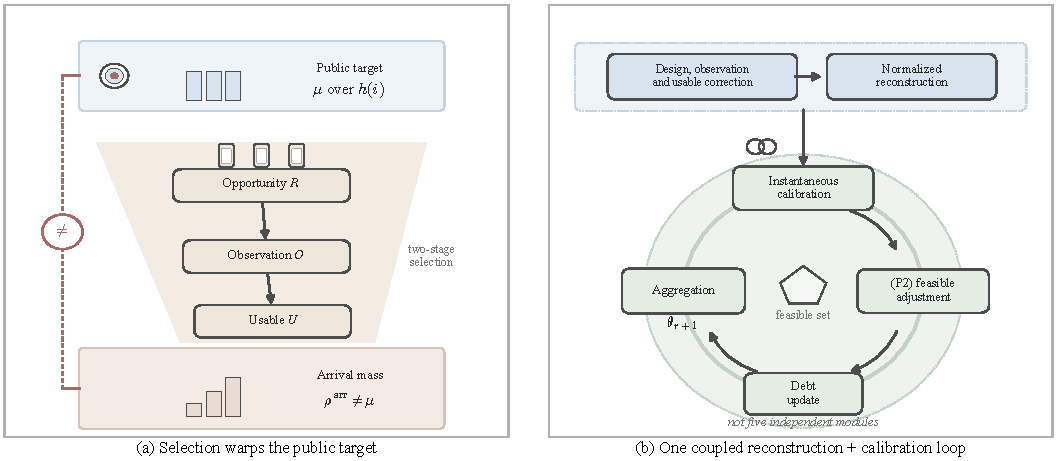
\includegraphics[width=\textwidth]{fig1_raven_problem_framework.pdf}
\caption{RAVEN-MCS aligns asynchronous federated completion with a public
deployment target.  (a)~The three selection layers within the two-stage MCS
process induce an arrival law that need not match the deployment target.
(b)~RAVEN-MCS reconstructs target-relevant mass and then calibrates it within the
currently feasible mobile support as one coordinated architecture, rather than
as five independent modules.  The feasibility program (P2) is defined in
Section~\ref{sec:calibration}.}
\label{fig:raven_overview}
\end{figure*}

Our main contributions are as follows.

\begin{itemize}
    \item \textbf{Deployment-target risk semantics under two-stage non-random
    selection.}
    We formulate asynchronous federated MCS completion as a
    deployment-target alignment problem rather than an arrival-centered
    learning problem.  The formulation distinguishes the atomic deployment law
    from the law induced by mobile opportunity, observation, and usable-update
    selection, and defines structural mismatch at both deployment-group and
    client--opportunity-stratum levels.  We prove that when the deployment and
    arrival laws differ, their induced risk functionals are not generally
    interchangeable.  This provides the formal basis for asking whether a model
    is trained for the population it is actually intended to serve.

    \item \textbf{Selection-layer-aware target reconstruction.}
    We develop an exposure-aware normalized reconstruction that keeps the
    opportunity/design, observation, and usable-update mechanisms separate
    instead of collapsing them into a single missingness probability.  The
    correction uses only legal pre-outcome information and local
    H\'ajek normalization, and yields a selection-corrected reference mass
    for aggregation.  Usable-update correction is retained as a third
    sequential factor, not as an isolated empirical driver.
    Under explicit support,
    sequential ignorability, correct ideal selection laws, and cluster-level
    regularity, we show that the ideal pooled normalized sequential estimator
    recovers the compatible deployment target.  Clipping is a finite-sample
    stabilizer, not an unbiasedness claim.  Design is applied when the
    public target has compatible support, and is withheld when it does
    not (SensorScope on, U-Air off).  A finite-sample aggregate coverage
    bound is analyzed separately and audited as a diagnostic in
    Section~\ref{subsec:eval_certificate}.

    \item \textbf{Feasibility-aware instantaneous and long-term target
    calibration.}
    We show that statistically reconstructed target mass and instantaneous
    mobile realizability are different problems.  RAVEN-MCS therefore
    calibrates the corrected reference inside the current feasible aggregation
    set while accounting for target mismatch, reference fidelity, uncertainty,
    and staleness, and carries unresolved group under-service through a
    long-term target-debt process.  The resulting calibration program has a
    nonempty compact convex feasible set and a unique global minimizer under the
    stated conditions.  When the active set is held fixed and target support is
    compatible, the implemented clipped plug-in is a Lipschitz perturbation of
    the same-window ideal reference, and P2 does not amplify that error.
    Target debt is an internal accounting recursion for residual
    group under-service, not a standalone performance contribution.
\end{itemize}

RAVEN's novelty is therefore not inverse-probability weighting or H\'ajek
normalization as such.  It is the combination of deployment-target semantics,
selection-layer legal histories, and finite-support calibration.
Isolated usable-update and debt terms are retained for sequential
factorization and accounting; they are not the empirical claim.

We evaluate these contributions with a no-harm control, a risk-semantic
block, SensorScope and U-Air reconstruction experiments under a protocol
selection process, and a T-Drive taxi opportunity replay that is not a
method ranking.  RAVEN-MCS uses support-conditional Design: on when
target support is compatible (SensorScope), off when it is not (U-Air).
Section~\ref{subsec:eval_certificate} additionally audits a candidate
per-window coverage Gate on a frozen coverage-stress oracle.  That Gate
is not used to switch Design in E3 or E4.

The remainder of the paper is organized as follows.
Section~\ref{sec:related_work} reviews sparse MCS completion, asynchronous
federated completion, participation-aware FL, and federated conformal
prediction.
Section~\ref{sec:system_model} formulates the two-stage, three-layer selection
process and deployment-target risk.
Sections~\ref{sec:reconstruction} and \ref{sec:calibration} present
selection-layer-aware reconstruction and feasibility-aware calibration,
respectively.
Section~\ref{sec:theory} presents the theoretical analysis.
Section~\ref{sec:evaluation} reports the evaluation.
Section~\ref{sec:discussion} discusses claim and modeling boundaries.
Section~\ref{sec:conclusion} concludes the paper.
Proofs and additional tables are in a separate supplemental file.


\section{Related Work}
\label{sec:related_work}

\subsection{Sparse Mobile Crowdsensing and Data Completion}

Sparse mobile crowdsensing reduces sensing cost by collecting only part of the
spatiotemporal field and inferring the unsensed portion
\cite{ganti2011mobile,guo2015mobile,ma2014opportunities}.  A substantial line of
work therefore focuses on exploiting spatial and temporal structure to improve
completion accuracy.  Wang \emph{et al.}~\cite{wang2023spatiotemporal} combine
graph modeling with spatiotemporal learning for joint urban inference and
prediction, while their outlier-aware completion method
\cite{wang2023outlier} exploits both intra- and inter-data correlations to
mitigate the effect of anomalous observations.  Transformer-style
spatiotemporal inference \cite{wang2023transformer} and few-shot completion for
new sensing tasks \cite{wang2024fewshot} further reduce dependence on dense
historical labels.  Li \emph{et al.}
\cite{li2024robust} jointly study adaptive region division, robust inference,
and cost-effective cell selection under sparse noise.  More recent approaches
model the evolutionary structure of sparse observations
\cite{wang2025evolutionary}, examine how sparse completion affects downstream
MCS tasks \cite{xu2025rethinking}, exploit cross-scale correlations through
a spatiotemporal pyramid \cite{liu2026pyramid}, address cold-start completion
with one-shot mapping transfer \cite{zhang2026mapt}, or price sparse sensing
data through uncertainty quantification \cite{liu2026pricing}.
Orthogonal MCS lines study worker recruitment and trust
\cite{liu2026multidimensional}, incentive and privacy mechanisms
\cite{zhang2025incentive,lu2025piece}, and locally private truth discovery
\cite{zhang2026locally}.  These studies substantially
advance completion, recruitment, pricing, or privacy, but their main objective
is not deployment-target risk under sequential selection.
In contrast, RAVEN-MCS asks a different question: when the data that become
available are themselves produced by non-random mobile opportunity and
observation processes, which population risk does the resulting training mass
represent?  This distinction motivates our explicit separation between the
deployment target $h(i)$ and the opportunity stratum $s(i)$, as well as the
deployment-target and arrival-risk semantics in Section~\ref{sec:system_model}.

\subsection{Federated and Asynchronous Data Completion}

Federated learning (FL) enables distributed clients to train a shared model
without centralizing their raw data, with FedAvg providing the canonical
model-averaging formulation \cite{mcmahan2017communication,yang2019federated}.
Surveys and open-problem statements further position FL as a privacy-preserving
distributed learning primitive
\cite{kairouz2021advances,li2020federated}.  This paradigm is
particularly attractive for MCS because sensing records are naturally
distributed across mobile participants.  Most closely related to our setting,
Wang \emph{et al.}~\cite{wang2026federated} develop a federated distributed
data-completion framework for sparse MCS, combining local completion models
with a time-aware architecture and asynchronous aggregation to accommodate
irregular client data.  Spatio-temporal-aware dynamic FL has also been studied
for spatial crowdsourcing \cite{li2026stdfl}.  In the broader asynchronous-FL
literature, FedAsync updates the server as client models arrive
\cite{xie2019asynchronous}, adaptive asynchronous aggregation addresses edge
dynamics and resource constraints
\cite{liu2023adaptive,sun2024staleness}, and recent staleness-aware designs
explicitly trade accuracy against system efficiency under heterogeneous client
speeds \cite{sun2024staleness}; most recently, semi-asynchronous aggregation
with adaptive weighting and selective training has been proposed to reduce
communication and computation cost \cite{islam2025seafl}.  These
works establish that privacy, distributed sparsity, and stale updates can be
handled without reverting to centralized completion.  Their primary focus,
however, is how to learn effectively from the updates that participate or
arrive.  RAVEN-MCS instead additionally models how sensing opportunities,
actual observations, and usable asynchronous updates sequentially determine
\emph{which} target mass reaches the server.  It therefore separates
statistical target reconstruction from the subsequent feasibility-aware
aggregation decision rather than treating asynchronous arrivals themselves as
the implicit deployment population.

Federated conformal prediction constructs distributed prediction sets
with coverage guarantees when client data are heterogeneous.
Lu \emph{et al.}~\cite{lu2023federated} use partial exchangeability to
extend split conformal prediction to federated models.
Plassier \emph{et al.}~\cite{plassier2023conformal} form importance-weighted
quantiles under label shift, with privacy constraints.
Both objects are label-set coverage for a trained predictor.
The diagnostic Gate in Section~\ref{subsec:agg_certificate_alg} is a
window-level lower bound on realized aggregate opportunity coverage
$C_t$, used only as an audit of a candidate Design switch, not as a
prediction set and not as the Design rule used in the reconstruction
experiments.

\subsection{Non-Uniform Participation and Selection Bias in FL}

A complementary FL literature studies partial and non-uniform client
participation.  Wang and Ji~\cite{wang2022unified} provide a unified convergence
analysis for arbitrary participation patterns.  FedVARP
\cite{jhunjhunwala2022fedvarp} reduces the optimization variance caused by
partial participation using server-side surrogate updates, whereas anchor
sampling \cite{wu2023anchor} is designed to improve learning under partial
client participation and data heterogeneity.  FedAU
\cite{wang2024lightweight} is particularly relevant: it estimates adaptive
aggregation weights from participation history so that heterogeneous,
unknown participation does not silently replace the original FL objective by
a participation-weighted one.  More directly related to temporal dependence,
Sun \emph{et al.}~\cite{sun2025debiasing} show that non-uniform, correlated
client availability can bias FedAvg and develop a debiasing method for
correlated participation.  Agnostic FL further asks the model to perform well
against an adversarially chosen mixture of client distributions
\cite{mohri2019agnostic}, while FedCure mitigates participation bias in
semi-asynchronous hierarchical FL \cite{chen2026fedcure}.  Heterogeneity-aware
optimization methods such as FedProx and SCAFFOLD
\cite{li2020fedprox,karimireddy2020scaffold} address client drift; more recent
participation-aware designs, including FedAU \cite{wang2024lightweight},
Sun \emph{et al.}~\cite{sun2025debiasing}, and FedCure \cite{chen2026fedcure},
recognize that the participating updates themselves may not represent the
population of interest.  Still, these works treat participation as the object
to be corrected, whereas RAVEN-MCS additionally separates the sensing-side
selection layers (opportunity and observation) from the update-side usable
selection.
Closest in the two-stage FL vocabulary is FedIPW
\cite{morishita2026who}, which factors population-level enrollment and then
round-level participation and reweights updates toward a target-population
mean client update.  That factorization is still on the client roster: who is
reachable for training, and who reports in a round.  It does not factor MCS
opportunity or observation of sensing units, and the aligned object is not a
public deployment measure over $h(i)$.  FedIPW's aggregate-calibration
extension also uses known population summaries to reweight an enrolled sample;
it is not a finite-window feasible-set program on currently usable MCS
clients.  We therefore cite FedIPW as the nearest enrollment--participation
IPW, not as an MCS completion baseline, and we do not run it as a comparator.
Classical survey estimators provide the inverse-probability and ratio-normalized
building blocks used by our H\'ajek-style baselines
\cite{horvitz1952generalization,hajek1971comment}.
Single-step covariate-shift likelihood weighting
\cite{shimodaira2000covariate} and sequential inverse-probability
estimation for missing regressors \cite{robins1994estimation} supply
the classical density-ratio and IPW vocabulary.
Importance weighting can also lose effect in over-parameterized
networks \cite{byrd2019importance}; that classification mechanism is
not claimed here.  RAVEN-MCS is not a
new IPW estimator: it uses sequential R/O/U legal histories and maps
the reconstructed reference onto a finite-window feasible set.

These results show that participation cannot always be treated as
uniform random sampling.  In FedAU in particular, participation can
change the effective FL objective.  RAVEN-MCS differs in the object
being aligned and in the selection process being modeled: the reference
is an application-level deployment target, whereas selection occurs
before and after local sensing rather than only at client enrollment or
update participation~\cite{morishita2026who}.  The problem studied here combines three selection
layers within a two-stage MCS process: mobile opportunity $R$,
observation $O$, and usable update $U$.  RAVEN-MCS fixes a deployment
target independently of this arrival process.  It reconstructs
target-relevant mass under stage-specific legal information boundaries
and then calibrates the reconstructed reference within the
time-varying feasible client support.  The distinguishing point is
therefore not inverse weighting or asynchronous aggregation in
isolation.  It is the joint \emph{deployment-target risk
semantics--selection-layer-aware reconstruction--feasibility-aware
calibration} chain required by mobile crowdsensing under non-random
sensing and update availability.  Table~\ref{tab:nearest_neighbor}
contrasts RAVEN-MCS with the nearest-neighbor method families on these
four axes.

\begin{table}[!t]
\centering
\caption{Nearest-neighbor comparison.  RAVEN's distinction is not IPW
itself, but a public deployment target, sequential R/O/U legal
histories, sensing-side correction, and finite-window calibration.
FedIPW~\cite{morishita2026who} is the nearest two-stage FL IPW
(enrollment then participation); it is not an MCS baseline.
Adapted FedAU/ObsUse used in Section~\ref{sec:evaluation} are
windowed implementations, not official reproductions.}
\label{tab:nearest_neighbor}
\setlength{\tabcolsep}{3.2pt}
{\footnotesize
\begin{tabular*}{\columnwidth}{@{\extracolsep{\fill}}p{1.42cm}p{1.28cm}p{1.18cm}p{1.12cm}p{1.42cm}}
\toprule
Family & Target & Selection & Sensing-side & Finite-support cal.\\
\midrule
Covariate-shift FL & target/test domain & sample/client & no & no\\
FedAU / participation debiasing & original FL objective & client participation & no & no\\
FedIPW & pop.\ mean update & enroll then participate & no & no\\
Correlated participation & long-run availability & client/update & no & limited\\
Agnostic / targeted FL & client mixture & client distribution & no & not the issue\\
Semi-async fairness/queue & participation fairness & client/update & no & queue \(\neq\) target debt\\
\textbf{RAVEN-MCS} & public deployment \(\mu\) & R/O/U & yes & yes\\
\bottomrule
\end{tabular*}}
\end{table}


\section{System Model and Target-Risk Formulation}
\label{sec:system_model}

\subsection{Windowed Asynchronous Mobile Crowdsensing}
\label{subsec:windowed_mcs}

We consider a mobile crowdsensing (MCS) system with a server and a set of
clients $\mathcal{K}=\{1,\ldots,K\}$.  The common prediction domain is
partitioned into atomic units $i\in\mathcal{I}$; an atomic unit may be written as
$i=(n,t)$, where $n$ is a spatial unit and $t$ is an absolute time index.  Unit
$i$ has deployment target $Y_i$ and public deployment context
$C_i^{\mathrm{dep}}$.  All clients contribute to a common predictor
$\widehat Y_i=f_{\theta}(i;C_i^{\mathrm{dep}})$.
A client-side observation of unit $i$ is denoted by $Z_{k,r,i}$ when it is
available to client $k$ in server window $r$.

Server time is divided into aggregation windows
$\mathcal{W}_r=[T_r,T_{r+1})$ for $r=0,1,\ldots$.
The server keeps $\theta_r$ fixed during $\mathcal{W}_r$.  Client $k$ may start
local training from a previously downloaded model $\theta_{\sigma_{k,r}}$,
where $\sigma_{k,r}\le r$.  We use
$\tau_{k,r}\triangleq r-\sigma_{k,r}$
as the model-version staleness of that attempt.  Updates may arrive at
different times within one window, but individual arrivals do not
immediately modify the global model.  The server closes the window,
determines which registered attempts are usable, computes one
aggregation vector, and then performs the single transition
$\theta_r\rightarrow\theta_{r+1}$.  This \emph{windowed-asynchronous}
semantics is distinct from immediate-update FedAsync, in which an
arrival would revise the global model before the window closes.  It
keeps exogenous mobile/update events independent of the method-specific
aggregation weights.

\subsection{Two-Stage, Three-Layer Non-Random Selection}
\label{subsec:selection_process}

The title's \emph{two-stage selection} consists of a sensing-side stage and an
update-side stage.  The sensing-side stage itself has two layers: mobile
opportunity and actual observation.  The update-side stage determines whether a
registered client attempt becomes usable before window closure.

For client $k$, window $r$, and unit $i$, let
$R_{k,r,i}\in\{0,1\}$ be the realized mobile opportunity indicator.
It indicates whether $(k,i)$ belongs to the opportunity/risk set in
window $r$ before the current sensing outcome is revealed.
Conditional on $R_{k,r,i}=1$,
$O_{k,r,i}\in\{0,1\}$
indicates whether unit $i$ is actually observed.  A client with a
nonempty observed buffer registers an update attempt; the set of
registered clients is $\mathcal{E}_r$.  For $k\in\mathcal{E}_r$, the
attempted update is usable ($U_{k,r}=1$) only if computation and
transmission succeed, the update arrives by $T_{r+1}$, and its
staleness satisfies $\tau_{k,r}\le S_{\max}$.  Otherwise,
$U_{k,r}=0$.  We first define the usable set
$\mathcal{U}_r\triangleq\{k\in\mathcal{E}_r:U_{k,r}=1\}$.
After target-relevant mass is reconstructed in
Section~\ref{sec:reconstruction}, zero-mass clients are removed and the
actual aggregation set $\mathcal{A}_r\subseteq\mathcal{U}_r$ is formed.
Failures, timeouts, network interruptions, and stale arrivals remain
recorded as $U_{k,r}=0$ rather than disappearing from the selection
log.

We distinguish two structural mappings: the \emph{deployment-target
group} $h(i)\in\mathcal{G}$ and the \emph{opportunity stratum}
$s(i)\in\mathcal{S}$.  The group mapping specifies which deployment
mass the predictor should serve, whereas the stratum mapping pools
repeatable mobile exposure patterns for selection modeling.  The two
mappings are different scientific objects, so $h(i)\neq s(i)$ in
general.  Both mappings are frozen from public/training-side
information and do not use test-label values.

For theoretical bookkeeping, let the normalized opportunity-event law in
window $r$ be
\begin{equation}
 P_r^{\mathrm{opp}}(k,i)
 =
 \pi^{\mathrm{opp}}_{k,s(i),r}
 \nu^{\mathrm{opp}}_{k,r}(i\mid s(i)),
 \qquad
 \sum_{k,i}P_r^{\mathrm{opp}}(k,i)=1,
 \label{eq:opp_event_law}
\end{equation}
where $\pi^{\mathrm{opp}}_{k,s,r}$ is the client--stratum opportunity mass and
$\nu^{\mathrm{opp}}_{k,r}(i\mid s)$ is the conditional atomic opportunity law.
The realized risk-set indicators $R_{k,r,i}$ are the implementation-level
bookkeeping of the opportunity events induced by this mobile exposure process;
they are not assumed to be mutually independent Bernoulli draws.

The subsequent selection probabilities are
\begin{align}
 p^{\mathrm{obs}}_{k,r,i}
 &\triangleq
 \Pr\!\left(
 O_{k,r,i}=1
 \mid
 R_{k,r,i}=1,\mathcal{H}^{\mathrm{obs}}_{k,r,i}
 \right),
 \label{eq:pobs_def}\\
 q^{\mathrm{use}}_{k,r}
 &\triangleq
 \Pr\!\left(
 U_{k,r}=1
 \mid
 k\in\mathcal{E}_r,\mathcal{H}^{\mathrm{use}}_{k,r}
 \right).
 \label{eq:quse_def}
\end{align}
The observation history $\mathcal{H}^{\mathrm{obs}}_{k,r,i}$ contains
only information available before $O_{k,r,i}$ is realized.  The
usable-update history $\mathcal{H}^{\mathrm{use}}_{k,r}$ is measured
after the sensing-side stage but before $U_{k,r}$ is realized.  It may
therefore contain the already observed registration state, but not the
realized computation/transmission outcomes, future events, or the
current update vector used for aggregation.  This sequential
information boundary is part of the statistical model.

\subsection{Public Deployment Target and Compatible Target Measures}
\label{subsec:target_measures}

We begin with a public, label-independent atomic deployment target
\begin{equation}
    \varpi_i^{\mathrm{tar}}\ge0,
    \qquad
    \sum_{i\in\mathcal{I}_{\mathrm{dep}}}
    \varpi_i^{\mathrm{tar}}=1.
    \label{eq:atomic_target}
\end{equation}
Its deployment-group marginal is
$\mu_g=\sum_{i:h(i)=g}\varpi_i^{\mathrm{tar}}$, so
$\boldsymbol{\mu}\in\Delta^{|\mathcal{G}|-1}$.
These quantities define the application-level target served by the deployed
predictor.

For opportunity correction we require a compatible client--stratum target.
First define the target mass of opportunity stratum $s$ by
\begin{equation}
    \Lambda_s^{\mathrm{tar}}
    =
    \sum_{i:s(i)=s}\varpi_i^{\mathrm{tar}}.
    \label{eq:target_stratum_mass}
\end{equation}
For $\Lambda_s^{\mathrm{tar}}>0$, define
\begin{equation}
    \nu^{\mathrm{tar}}_{i\mid s}
    =
    \frac{\varpi_i^{\mathrm{tar}}}
         {\Lambda_s^{\mathrm{tar}}},
    \qquad s(i)=s,
    \label{eq:target_conditional_atomic}
\end{equation}
and let $\lambda^{\mathrm{tar}}_{k\mid s}\ge0$ be a frozen, public,
support-compatible target client share satisfying
$\sum_k\lambda^{\mathrm{tar}}_{k\mid s}=1$.
For a zero-target stratum $\Lambda_s^{\mathrm{tar}}=0$, all atomic target
masses in that stratum are zero by \eqref{eq:target_stratum_mass} and
nonnegativity.  We therefore set its client--stratum and client--atomic target
masses to zero and do not evaluate $\nu^{\mathrm{tar}}_{i\mid s}$ or
$\lambda^{\mathrm{tar}}_{k\mid s}$.  Formally,
\begin{equation}
 \pi^{\mathrm{tar}}_{k,s}
 =
 \begin{cases}
 \Lambda_s^{\mathrm{tar}}\lambda^{\mathrm{tar}}_{k\mid s},
 & \Lambda_s^{\mathrm{tar}}>0,\\
 0, & \Lambda_s^{\mathrm{tar}}=0,
 \end{cases}
 \label{eq:target_ks_mass}
\end{equation}
and
\begin{equation}
 \pi^{\mathrm{tar}}_{k,i}
 =
 \begin{cases}
 \pi^{\mathrm{tar}}_{k,s(i)}
 \nu^{\mathrm{tar}}_{i\mid s(i)},
 & \Lambda_{s(i)}^{\mathrm{tar}}>0,\\
 0, & \Lambda_{s(i)}^{\mathrm{tar}}=0.
 \end{cases}
 \label{eq:target_ki_mass}
\end{equation}
By construction,
\begin{equation}
    \sum_k\pi^{\mathrm{tar}}_{k,i}
    =
    \varpi_i^{\mathrm{tar}},
    \qquad
    \sum_{k,s}\pi^{\mathrm{tar}}_{k,s}=1.
    \label{eq:target_compatibility}
\end{equation}
Equation~\eqref{eq:target_compatibility} is the compatibility bridge between the
deployment-risk target and the client--stratum target used for selection
reconstruction.  All target quantities are frozen before test-label evaluation.

\subsection{Aggregate Coverage Certification Object}
\label{subsec:agg_coverage_object}

RAVEN-MCS applies Design when the public target has compatible support.
Separately, a finite-sample certification object is the scalar realized
aggregate coverage
\begin{equation}
 C_t
 =
 \sum_{i\in I_{\mathrm{tar}}}
 \pi_i^{\mathrm{tar}}
 \,
 1\!\left\{\pi_{i,t}^{\mathrm{opp}}\ge\pi_{\mathrm{safe}}\right\},
 \label{eq:agg_Ct}
\end{equation}
where $I_{\mathrm{tar}}$ is the frozen target-positive pair index set,
$\sum_{i\in I_{\mathrm{tar}}}\pi_i^{\mathrm{tar}}=1$ up to numerical tolerance,
$\pi_{i,t}^{\mathrm{opp}}$ is the realized opportunity quantity of pair $i$ in
window $t$, and $\pi_{\mathrm{safe}}$ is a frozen public positivity threshold.
Thus $C_t\in[0,1]$.  This $C_t$ is distinct from the
deployment context $C_i^{\mathrm{dep}}$ and from the feasible set
$\mathcal{C}_r$.  The coverage condition studied below is
$C_t\ge\tau_{\mathrm{cov}}$ with $\tau_{\mathrm{cov}}=0.05$.

Realized coverage $C_t$ is an outcome available only after window $t$
closes.  The predictor $\widehat C_t=f_t(F_{t-})$ is any
$F_{t-}$-measurable forecast; it is not a certificate.  The certified
scalar is the lower bound $C^{\mathrm{LCB}}_t$ of
Section~\ref{subsec:agg_certificate_alg}.  A diagnostic Gate compares
$C^{\mathrm{LCB}}_t$ with $\tau_{\mathrm{cov}}$, never $\widehat C_t$
with $\tau_{\mathrm{cov}}$.  That Gate does not switch Design in
Algorithm~\ref{alg:window_close}.

\subsection{Deployment-Target Risk Versus Arrival Risk}
\label{subsec:target_risk}

For a loss $\ell(\widehat Y,Y)$, the deployment-target risk is
\begin{equation}
 \mathcal{R}_{\mu}(\theta)
 =
 \sum_{i\in\mathcal{I}_{\mathrm{dep}}}
 \varpi_i^{\mathrm{tar}}
 \ell\!\left(
 f_{\theta}(i;C_i^{\mathrm{dep}}),Y_i
 \right).
 \label{eq:target_risk}
\end{equation}
By contrast, the data reaching learning are distributed according to the
opportunity, observation, and usable-update mechanisms.

For evaluation, quantities without a window index denote the frozen
evaluation-period marginals of their corresponding pre-outcome mechanisms.
Thus a label-free atomic arrival intensity is
\begin{equation}
 \widehat r_i^{\mathrm{arr}}
 =
 \sum_k
 \widehat\pi^{\mathrm{opp}}_{k,s(i)}
 \widehat\nu^{\mathrm{opp}}_{k}(i\mid s(i))
 \widehat p^{\mathrm{obs}}_{k,i}
 \widehat q^{\mathrm{use}}_{k,s(i)},
 \label{eq:arrival_intensity}
\end{equation}
where $\widehat q^{\mathrm{use}}_{k,s}$ is the corresponding
evaluation-period marginal of the legal pre-$U$ usable-update model over
registered attempts associated with stratum $s$.  Normalize
\begin{equation}
 \widetilde\rho_i^{\mathrm{arr}}
 =
 \frac{\widehat r_i^{\mathrm{arr}}}
 {\sum_{j\in\mathcal{I}_{\mathrm{dep}}}\widehat r_j^{\mathrm{arr}}},
 \label{eq:arrival_distribution}
\end{equation}
and define
\begin{equation}
 \mathcal{R}_{\rho}(\theta)
 =
 \sum_{i\in\mathcal{I}_{\mathrm{dep}}}
 \widetilde\rho_i^{\mathrm{arr}}
 \ell\!\left(
 f_{\theta}(i;C_i^{\mathrm{dep}}),Y_i
 \right).
 \label{eq:arrival_risk}
\end{equation}
The two risks answer different questions.  RAVEN-MCS therefore treats
deployment-target alignment, rather than usable-update frequency, as the
reference semantics of the learning problem.

\subsection{Structural Alignment Objective}
\label{subsec:design_objective}

Section~\ref{sec:reconstruction} will construct two corrected within-client
compositions: a deployment-group composition
$\mathbf{c}^{g}_{k,r}\in\Delta^{|\mathcal{G}|-1}$ and an opportunity-stratum
composition $\mathbf{c}^{s}_{k,r}\in\Delta^{|\mathcal{S}|-1}$.  For the final
aggregation set $\mathcal{A}_r$, define
$M_r=[\mathbf{c}^{g}_{k,r}]_{k\in\mathcal{A}_r}$.
Given feasible aggregation weights $\boldsymbol\alpha_r$, the effective
deployment-group composition in an active window is
$\boldsymbol\omega_r=M_r\boldsymbol\alpha_r$.

Let $\eta_r>0$ denote the server step size and define
$I_r=\mathbf{1}\{|\mathcal{A}_r|>0\}$ and
$S_R=\sum_{r=0}^{R-1}\eta_r I_r$.
For $S_R>0$,
\begin{equation}
    \overline{\boldsymbol\omega}_R
    =
    \frac{1}{S_R}
    \sum_{r=0}^{R-1}
    \eta_r I_r\boldsymbol\omega_r.
    \label{eq:omega_bar}
\end{equation}
The group-level structural mismatch is
$\Delta_{\mathrm{group}}(R)=\left\|
\overline{\boldsymbol\omega}_R-\boldsymbol\mu
\right\|_1$.

For client--stratum structure, extend $\alpha_{k,r}=0$ to
$k\notin\mathcal{A}_r$ and define
\begin{equation}
 \widehat\Pi_{k,s}(R)
 =
 \frac{1}{S_R}
 \sum_{r=0}^{R-1}
 \eta_r I_r\,
 \alpha_{k,r}\,
 c^{s}_{k,r,s}.
 \label{eq:Pi_hat_ks}
\end{equation}
Because each active-window $\boldsymbol\alpha_r$ and each
$\mathbf{c}^{s}_{k,r}$ are probability vectors,
$\sum_{k,s}\widehat\Pi_{k,s}(R)=1$.  We therefore measure
\begin{equation}
 \Delta_{c\text{-}s}(R)
 =
 \sum_{k,s}
 \left|
 \widehat\Pi_{k,s}(R)-\pi^{\mathrm{tar}}_{k,s}
 \right|.
 \label{eq:delta_cs}
\end{equation}
The overall design goal is to keep $\mathcal{R}_{\mu}$ low while
reducing $\Delta_{\mathrm{group}}$ and $\Delta_{c\text{-}s}$ under
time-varying mobile feasibility and legal pre-outcome information.


\section{Selection-Layer-Aware Target Reconstruction}
\label{sec:reconstruction}

RAVEN-MCS (Risk Alignment Via Exposure-aware Normalization) first reconstructs
which deployment-relevant mass the usable data represent.  Opportunity,
observation, and usable-update selection are kept separate because they have
different conditioning sets and therefore cannot be replaced by a single
generic missingness probability.

\subsection{Opportunity/Design Correction}
\label{subsec:design_correction}

For a target-supported client--atomic pair, the ideal opportunity/design ratio is
\begin{equation}
 \zeta^{o}_{k,r,i}
 =
 \frac{\pi^{\mathrm{tar}}_{k,s(i)}}
      {\pi^{\mathrm{opp}}_{k,s(i),r}}
 \frac{\nu^{\mathrm{tar}}_{i\mid s(i)}}
      {\nu^{\mathrm{opp}}_{k,r}(i\mid s(i))}
 =
 \frac{\pi^{\mathrm{tar}}_{k,i}}
      {P_r^{\mathrm{opp}}(k,i)}.
 \label{eq:design_ratio_general}
\end{equation}
Under the within-stratum exchangeability used by the main protocol,
$\nu^{\mathrm{opp}}_{k,r}(i\mid s)=\nu^{\mathrm{tar}}_{i\mid s}$, this reduces to
\begin{equation}
 \widehat\zeta^{o}_{k,r,s}
 =
 \frac{\pi^{\mathrm{tar}}_{k,s}}
 {\max\{\widehat\pi^{\mathrm{opp}}_{k,s,r},\pi_{\min}\}}.
 \label{eq:design_ratio_simple}
\end{equation}
The opportunity estimate is lagged: current-window outcomes cannot alter the
weight applied to that same window.  One admissible implementation uses
\begin{align*}
 C^{\mathrm{opp}}_{k,s,r}
 &=
 \rho_{\mathrm{opp}}C^{\mathrm{opp}}_{k,s,r-1}
 +N^{\mathrm{opp}}_{k,s,r-1},\\
 \widehat\pi^{\mathrm{opp}}_{k,s,r}
 &=
 \frac{C^{\mathrm{opp}}_{k,s,r}+\epsilon_{\mathrm{opp}}}
 {\sum_{j,u}
 (C^{\mathrm{opp}}_{j,u,r}+\epsilon_{\mathrm{opp}})}.
\end{align*}
Other pre-outcome estimators are compatible with the framework if they preserve
the same support and information boundary.

\subsection{Observation Correction and Local H\'ajek Normalization}
\label{subsec:observation_hajek}

The ideal first-stage weight for a realized opportunity is
$a^\star_{k,r,i}=\zeta^{o}_{k,r,i}/p^{\mathrm{obs}}_{k,r,i}$.
The implemented plug-in weight is stabilized as
\begin{equation}
 a_{k,r,i}
 =
 \min\!\left\{
 a_{\max},
 \frac{\widehat\zeta^{o}_{k,r,i}}
 {\max\{\widehat p^{\mathrm{obs}}_{k,r,i},p_{\min}\}}
 \right\}.
 \label{eq:a_stabilized}
\end{equation}
Define the corrected total mass
\begin{equation}
    m_{k,r}
    =
    \sum_i
    R_{k,r,i}O_{k,r,i}a_{k,r,i},
    \label{eq:m_total}
\end{equation}
the corrected deployment-group mass
\begin{equation}
 m^{g}_{k,r,g}
 =
 \sum_i
 R_{k,r,i}O_{k,r,i}a_{k,r,i}
 \mathbf{1}\{h(i)=g\},
 \label{eq:m_group}
\end{equation}
and the corrected opportunity-stratum mass
\begin{equation}
 m^{s}_{k,r,s}
 =
 \sum_i
 R_{k,r,i}O_{k,r,i}a_{k,r,i}
 \mathbf{1}\{s(i)=s\}.
 \label{eq:m_stratum}
\end{equation}
RAVEN aggregates only target-relevant usable clients:
$\mathcal{A}_r\triangleq\{k\in\mathcal{U}_r:m_{k,r}>0\}$.
Every $k\in\mathcal{A}_r$ has well-defined normalized record weights
$\overline a_{k,r,i}=\frac{R_{k,r,i}O_{k,r,i}a_{k,r,i}}{m_{k,r}}$.
Its deployment-group composition is
$c^{g}_{k,r,g}=\frac{m^{g}_{k,r,g}}{m_{k,r}}$, and its
opportunity-stratum composition is
$c^{s}_{k,r,s}=\frac{m^{s}_{k,r,s}}{m_{k,r}}$.
Both composition vectors sum to one for $k\in\mathcal{A}_r$.

The local effective sample size is
\begin{equation}
 n^{\mathrm{eff}}_{k,r}
 =
 \frac{m_{k,r}^2}
 {\sum_i
  (R_{k,r,i}O_{k,r,i}a_{k,r,i})^2}
 =
 \frac{1}{\sum_i\overline a_{k,r,i}^2}.
 \label{eq:neff}
\end{equation}
It measures weight concentration and is deliberately distinct from the
target-equivalent corrected mass $m_{k,r}$.

The local completion objective is
\begin{equation}
 \widehat F^{H}_{k,r}(\theta)
 =
 \sum_i
 \overline a_{k,r,i}
 \frac{1}{2}
 \left(
 f_{\theta}(i;C_i^{\mathrm{dep}})
 -
 Z_{k,r,i}
 \right)^2.
 \label{eq:local_hajek_objective}
\end{equation}
Starting from $\theta_{\sigma_{k,r}}$, client $k$ performs
$E_{\mathrm{loc}}$ local steps with step size $\gamma_r$.  Its normalized model
displacement is
\begin{equation}
 \mathbf{u}_{k,r}
 =
 \frac{
 \theta_{\sigma_{k,r}}
 -
 \theta^{(E_{\mathrm{loc}})}_{k,r}
 }{\gamma_r E_{\mathrm{loc}}}.
 \label{eq:normalized_update}
\end{equation}

\subsection{Usable-Update Correction and Reference Aggregation Mass}
\label{subsec:usable_correction}

For a registered attempt, $\widehat q^{\mathrm{use}}_{k,r}$ is estimated only
from variables measurable before $U_{k,r}$ is realized.  For
$k\in\mathcal{A}_r$, define
\begin{equation}
 d_{k,r}
 =
 \min\!\left\{
 d_{\max},
 \frac{1}
 {\max\{\widehat q^{\mathrm{use}}_{k,r},q_{\min}\}}
 \right\},
 \label{eq:d_use}
\end{equation}
and $b_{k,r}=m_{k,r}d_{k,r}$.
The selection-corrected reference aggregation vector is
\begin{equation}
 \widehat\beta_{k,r}
 =
 \frac{b_{k,r}}
 {\sum_{j\in\mathcal{A}_r}b_{j,r}},
 \qquad
 k\in\mathcal{A}_r.
 \label{eq:beta_ref}
\end{equation}
Thus $\widehat{\boldsymbol\beta}_r$ is a probability vector on
$\mathcal{A}_r$.

To separate the exact statistical identity from its stabilized implementation,
define the ideal untruncated quantities
\begin{align*}
 m^\star_{k,r}
 &=
 \sum_i
 R_{k,r,i}O_{k,r,i}a^\star_{k,r,i},\\
 \overline a^\star_{k,r,i}
 &=
 \frac{
 R_{k,r,i}O_{k,r,i}a^\star_{k,r,i}
 }{m^\star_{k,r}},\\
 d^\star_{k,r}
 &=
 \frac{1}{q^{\mathrm{use}}_{k,r}},\\
 \beta^\star_{k,r}
 &=
 \frac{
 U_{k,r}m^\star_{k,r}d^\star_{k,r}
 }{
 \sum_j U_{j,r}m^\star_{j,r}d^\star_{j,r}
 }.
\end{align*}
For every target-relevant delivered record,
\begin{equation}
 \beta^\star_{k,r}\overline a^\star_{k,r,i}
 \propto
 R_{k,r,i}O_{k,r,i}U_{k,r}
 \frac{\zeta^{o}_{k,r,i}}
 {p^{\mathrm{obs}}_{k,r,i}q^{\mathrm{use}}_{k,r}}.
 \label{eq:factorized_global_weight}
\end{equation}
Equation~\eqref{eq:factorized_global_weight} is an identity for the
ideal untruncated construction.  The implemented
$\widehat{\boldsymbol\beta}_r$ and $\overline a_{k,r,i}$ are stabilized
plug-in counterparts.  They are not claimed to preserve exact
unbiasedness when clipping is active.

The corrected deployment-group composition represented by the usable
data before server calibration is
$\boldsymbol\omega_r^{\mathrm{ref}}=M_r\widehat{\boldsymbol\beta}_r$.
Even a statistically valid reconstruction need not satisfy
$\boldsymbol\omega_r^{\mathrm{ref}}=\boldsymbol\mu$ in a finite mobile
window.  The current feasible client set can lack target support.

\subsection{Information Boundary and Stabilization}
\label{subsec:information_boundary}

Every correction applied in window $r$ is measurable before its own random
outcome.  Opportunity estimates use lagged opportunity history,
observation propensities exclude the current sensing outcome and label,
and usable-update propensities exclude the realized $U$ outcome and
future events.  The server determines $\boldsymbol\alpha_r$ without
inspecting the coordinates, norm, or direction of a current random
update for the purpose of assigning that update's weight.  The clipping
constants in \eqref{eq:a_stabilized} and \eqref{eq:d_use} are
finite-sample bias--variance stabilizers.  Exact identification in
Section~\ref{sec:theory} concerns the ideal ratios, or equivalently
regimes in which the stabilizing bounds are inactive on target support.

\subsection{Why Pairwise Positive Lower Bounds Are Not the Formal Certificate}
\label{subsec:pairwise_barrier}

A previous certificate architecture formed a deterministic pre-window lower
bound $\underline{\pi}_{i,t}=L_i(F_{t-})$ for many target pairs simultaneously
and certified target mass only when $\underline{\pi}_{i,t}\ge\pi_{\mathrm{safe}}$.
That construction is structurally vacuous under hidden zero-opportunity events.
Proposition~\ref{prop:pairwise-lcb-barrier} shows that if
$P(X_t=0\mid F_{t-})>\alpha$ for a pair's opportunity $X_t$, then no strictly
positive deterministic $1-\alpha$ lower bound exists.  Corollary~\ref{cor:availability-barrier}
specializes the barrier to scenario-level availability retention $a<1-\alpha$.
For $\alpha=0.05$ the frozen stress levels $a\in\{0.80,0.60,0.40,0.20\}$ all
lie in that region.

Pairwise simultaneous positive LCBs may remain as motivation, a diagnostic
appendix, or a negative-result discussion.  They are not the aggregate
coverage object of \eqref{eq:agg_Ct} and are not used to switch Design.


\section{Feasibility-Aware Target Calibration}
\label{sec:calibration}

Selection reconstruction determines what the usable data statistically
represent.  It does not guarantee that the intended deployment target is
instantaneously realizable from the currently available clients.  RAVEN
therefore treats $\widehat{\boldsymbol\beta}_r$ as a corrected reference and
calibrates it within the support feasible at window closure.

\subsection{Feasible Aggregation Set}
\label{subsec:feasible_set}

Let $K_r=|\mathcal{A}_r|$ in an active window and retain
$M_r=[\mathbf{c}^{g}_{k,r}]_{k\in\mathcal{A}_r}$.  The server chooses
$\boldsymbol\alpha_r\in\mathbb{R}^{K_r}$ from
\begin{equation}
 \mathcal{C}_r
 =
 \left\{
 \boldsymbol\alpha:
 \mathbf{1}^{\top}\boldsymbol\alpha=1,\;
 0\le\alpha_k\le\overline\alpha_r,\;
 \|\boldsymbol\alpha\|_2^2\le\frac{1}{\overline E_r}
 \right\},
 \label{eq:Cr}
\end{equation}
where
\begin{equation}
\begin{aligned}
 \overline\alpha_r
 &=
 \min\!\left\{
 1,
 \max\!\left\{
 \alpha_{\max},
 \frac{1}{K_r}
 \right\}
 \right\},\\
 \overline E_r
 &=
 \min\{E_{\min},K_r\}.
\end{aligned}
 \label{eq:cap_ess}
\end{equation}
Here $0<\alpha_{\max}\le1$ and $E_{\min}\ge1$ are frozen design parameters.
The coordinate cap controls single-client dominance, while the
$\ell_2$ constraint imposes a minimum effective aggregation support.  The
uniform vector $\mathbf{1}/K_r$ belongs to $\mathcal{C}_r$, so every active
window has at least one feasible aggregation vector.

RAVEN also uses pre-aggregation uncertainty only.  A lagged variance proxy is
\begin{equation}
 v_{k,r}
 =
 \frac{
 \overline S_{k,r^-}^{\,2}
 }{
 \max\{n^{\mathrm{eff}}_{k,r},1\}
 }
 +
 v_{\mathrm{floor}},
 \qquad
 V_r=\operatorname{diag}(v_{k,r})\succeq0,
 \label{eq:variance_proxy}
\end{equation}
where $\overline S_{k,r^-}^{\,2}$ is available before the current random update
is weighted.  Let $\overline{\boldsymbol\tau}_r\ge0$ denote the frozen
pre-aggregation staleness vector.

\subsection{Long-Term Target Debt}
\label{subsec:debt}

Finite-window feasibility can make
$M_r\boldsymbol\alpha=\boldsymbol\mu$ impossible.  RAVEN maintains a
nonnegative target-debt vector
$\mathbf{Q}_r\in\mathbb{R}^{|\mathcal{G}|}_+$, initialized by
$\mathbf{Q}_0=\mathbf{0}$.  In an active window,
$\mathbf{Q}_{r+1}=\left[\mathbf{Q}_r+\eta_r(\boldsymbol\mu-\boldsymbol\omega_r)\right]_+$,
with $\boldsymbol\omega_r=M_r\boldsymbol\alpha_r$.
If the window is inactive, $\mathbf{Q}_{r+1}=\mathbf{Q}_r$.  A positive
$Q_{r,g}$ records accumulated under-service of deployment group $g$ without
pretending that unavailable target mass can be synthesized in the current
window.

For every prefix with $S_R>0$, the recursion implies the deterministic
accounting relation
\begin{equation}
 \left\|
 \overline{\boldsymbol\omega}_R-\boldsymbol\mu
 \right\|_1
 \le
 \frac{
 2\|\mathbf{Q}_R\|_1
 }{S_R}.
 \label{eq:debt_bound}
\end{equation}
The full derivation is given in the supplemental material.  This relation connects
bounded long-term debt to structural target mismatch.  It does not
claim that the debt component must have a large empirical effect in
every dataset.

\subsection{Feasibility-Aware Calibration Program}
\label{subsec:P2}

For every active window, RAVEN solves
$\text{(P2)}\ \min_{\boldsymbol\alpha\in\mathcal{C}_r}J_r(\boldsymbol\alpha)$.
The objective is
\begin{align}
 J_r(\boldsymbol\alpha)
 ={}&-\mathbf{Q}_r^{\top}M_r\boldsymbol\alpha
 +\frac{\lambda_g}{2}
 \|M_r\boldsymbol\alpha-\boldsymbol\mu\|_2^2
 \nonumber\\
 &+\frac{\lambda_{\beta}}{2}
 \|\boldsymbol\alpha-\widehat{\boldsymbol\beta}_r\|_2^2
 \nonumber\\
 &+\frac{\lambda_v}{2}
 \boldsymbol\alpha^{\top}V_r\boldsymbol\alpha
 +\lambda_s\overline{\boldsymbol\tau}_r^{\top}\boldsymbol\alpha.
\label{eq:P2_objective}
\end{align}
The debt term prioritizes accumulated under-served groups, and the
group term reduces instantaneous deployment mismatch.  The reference
term keeps calibration anchored to the selection-corrected mass.  The
variance term discourages concentrated uncertain updates, and the
staleness term penalizes old usable updates.  These are coordinated
terms of one calibration mechanism rather than five independent
innovations.

The distinction between
$\widehat{\boldsymbol\beta}_r$ and $\boldsymbol\alpha_r$ is fundamental.
$\widehat{\boldsymbol\beta}_r$ answers \emph{what the usable data
represent after sequential selection correction}.  $\boldsymbol\alpha_r$
answers \emph{what can be feasibly aggregated now while tracking the
deployment target}.  The former is statistical reconstruction; the
latter is mobile-feasibility-aware realization.

\subsection{Global Update and Window Logic}
\label{subsec:global_update}

Let $\boldsymbol\alpha_r^\star$ denote the solution of (P2).  The server update
is
\begin{equation}
 \theta_{r+1}
 =
 \theta_r
 -
 \eta_r
 \sum_{k\in\mathcal{A}_r}
 \alpha^\star_{k,r}\mathbf{u}_{k,r}.
 \label{eq:server_update}
\end{equation}
After aggregation, the server updates the debt via
$\mathbf{Q}_{r+1}=\left[\mathbf{Q}_r+\eta_r(\boldsymbol\mu-\boldsymbol\omega_r)\right]_+$,
where $\boldsymbol\omega_r=M_r\boldsymbol\alpha_r$.  It then advances all
lagged selection/variance states.  If
$\mathcal{A}_r=\varnothing$, the window is inactive.  In that case
$\theta_{r+1}=\theta_r$ and $\mathbf{Q}_{r+1}=\mathbf{Q}_r$, and the window
does not contribute to $S_R$.  Algorithm~\ref{alg:window_close}
records this window-close order.  The operational sequence is therefore
threefold: layered reconstruction yields the corrected reference weights
$\widehat{\boldsymbol\beta}_r$; the calibration program (P2) then produces the
feasible aggregation weights $\boldsymbol\alpha_r^\star$; finally, aggregation
and the debt update are performed.

\subsection{Finite-Sample Aggregate Coverage Certificate}
\label{subsec:agg_certificate_alg}

The Design-enabled reconstruction uses lagged opportunity ratios when
target support is compatible.  Separately, a candidate coverage Gate uses
only legal pre-window information $F_{t-}$.  Forbidden
inputs include the current availability mask, current entity identities,
current $R/O/U$, current $\pi^{\mathrm{opp}}$, current $C_t$, current
oracle-safe labels, and future windows.  Allowed inputs include lagged
realized $C_j$ for completed windows $j<t$, rolling historical summaries,
public time context, and the public scenario-level retention $a_t$.

Let $\widehat C_t=f_t(F_{t-})$ and define the one-sided residual
\begin{equation}
 S_t=\widehat C_t-C_t.
 \label{eq:agg_St}
\end{equation}
For a certified stable regime $g$, the calibration scores
$S_{j_1},\ldots,S_{j_n}$ are strictly historical and belong to the same
pre-registered regime.  Sort them as $S_{(1)}\le\cdots\le S_{(n)}$ and set
\begin{equation}
 k_n=\lceil(n+1)(1-\alpha)\rceil,
 \qquad
 \alpha=0.05.
 \label{eq:agg_kn}
\end{equation}
A finite empirical order statistic exists without clipping if and only if
$k_n\le n$, equivalently $n\ge\lceil 1/\alpha\rceil-1$.  Hence
$n_{\min}=19$.  The implementation must not clip $k_n$ to $n$ and still call
the result a nominal $95\%$ conformal certificate.  In particular $n=8$ is
not sufficient for that claim.

The certificate has three exclusive states.  In WARMUP, $n<19$ or no
finite $q_t$ exists: $C^{\mathrm{LCB}}_t=0$ and $\mathrm{Gate}_t$ is OFF.
RESET is triggered only after a completed CERTIFIED window with
$C^{\mathrm{LCB}}>C$: that window is retained as CERTIFIED, the next
window is RESET with $\mathrm{Gate}_t$ OFF, a new predictor snapshot
$f_{b+1}$ may be fit on completed past data only and then frozen, and
the calibration buffer is cleared.  In CERTIFIED, $n\ge 19$ and the same frozen
$f_b$ is used.  Operational CERTIFIED does not prove exchangeability; it
only defines the pre-registered subset of windows for which
Assumption~\ref{ass:score-exchangeability} is posited.
Theorem~\ref{thm:agg-lcb} remains conditional on that assumption even when
the algorithmic state is CERTIFIED.  Then $q_t=S_{(k_n)}^{\mathrm{cal}}$,
\begin{equation}
 C^{\mathrm{LCB}}_t=\max\{0,\widehat C_t-q_t\},
 \label{eq:agg_CLCB}
\end{equation}
and
\begin{equation}
 \mathrm{Gate}_t=1\{C^{\mathrm{LCB}}_t\ge\tau_{\mathrm{cov}}\}.
 \label{eq:agg_Gate}
\end{equation}
Algorithm~\ref{alg:agg_certificate} produces that Gate.  The finite-sample
guarantee applies only within certified stable regimes.  Unannounced regime
shifts outside this condition are an applicability boundary.  After a
completed CERTIFIED miscoverage, the certificate abstains until sufficient
calibration evidence is re-established.  Each certified calibration block $b$ uses a frozen
predictor snapshot $f_b$.  Within WARMUP and CERTIFIED of that block, the
scoring rule is not retrained.  Refit is allowed only after RESET, using
completed past data, after which the buffer is cleared and WARMUP restarts
until $n\ge 19$.  The current window is never used to form its own $q_t$.
Window-close RAVEN-MCS (Algorithm~\ref{alg:window_close}) applies Design by
target-support compatibility, not by $\mathrm{Gate}_t$.

\begin{algorithm}[t]
\caption{Aggregate coverage certificate (diagnostic Gate)}
\label{alg:agg_certificate}
\begin{algorithmic}[1]
\REQUIRE legal $F_{t-}$; public $a_t$; block snapshot $f_b$; same-block scores;
previous CERTIFIED miscoverage flag; $\alpha=0.05$; $\tau_{\mathrm{cov}}=0.05$; $n_{\min}=19$
\ENSURE $\mathrm{state}\in\{\mathrm{WARMUP},\mathrm{CERTIFIED},\mathrm{RESET}\}$,
block\_id, predictor\_snapshot\_id, $\widehat C_t$, $n$, $q_t$ if CERTIFIED,
$C^{\mathrm{LCB}}_t$, $\mathrm{Gate}_t$
\IF{the previous completed CERTIFIED window satisfied $C^{\mathrm{LCB}}>C$}
\STATE $\mathrm{state}\leftarrow\mathrm{RESET}$, $\mathrm{Gate}_t\leftarrow\mathrm{OFF}$
\STATE Fit $f_{b+1}$ on completed past data only; freeze it; clear the buffer
\STATE $\mathrm{state}\leftarrow\mathrm{WARMUP}$
\ELSE
\STATE Use the frozen snapshot $f_b$ of the current block
\IF{$n<19$ or $k_n>n$}
\STATE $\mathrm{state}\leftarrow\mathrm{WARMUP}$
\STATE $C^{\mathrm{LCB}}_t\leftarrow 0$, $\mathrm{Gate}_t\leftarrow\mathrm{OFF}$
\ELSE
\STATE $\mathrm{state}\leftarrow\mathrm{CERTIFIED}$ \COMMENT{scope; does not prove Assumption A}
\STATE $\widehat C_t\leftarrow f_b(F_{t-})$
\STATE $q_t\leftarrow S_{(k_n)}^{\mathrm{cal}}$ \COMMENT{no clipping of $k_n$ to $n$}
\STATE $C^{\mathrm{LCB}}_t\leftarrow\max\{0,\widehat C_t-q_t\}$
\STATE $\mathrm{Gate}_t\leftarrow 1\{C^{\mathrm{LCB}}_t\ge\tau_{\mathrm{cov}}\}$
\ENDIF
\ENDIF
\end{algorithmic}
\end{algorithm}

\begin{algorithm}[t]
\caption{Window-close RAVEN-MCS aggregation with support-conditional Design}
\label{alg:window_close}
\begin{algorithmic}[1]
\REQUIRE window $t$; recorded $R_{k,t,i}$, $O_{k,t,i}$, $U_{k,t}$;
public $\boldsymbol\mu$; debt $\mathbf{Q}_t$; model $\theta_t$;
frozen target-support compatibility
\ENSURE $\theta_{t+1}$, $\mathbf{Q}_{t+1}$, $\mathrm{Design}_t$
\STATE Form $\mathcal{E}_t$ and
$\mathcal{U}_t=\{k\in\mathcal{E}_t:U_{k,t}=1\}$.
\IF{the frozen public target is support-compatible}
\STATE $\mathrm{Design}_t\leftarrow\mathrm{ON}$
\STATE Compute lagged opportunity/design ratios
$\widehat\zeta^{o}_{k,t,i}$.
\ELSE
\STATE $\mathrm{Design}_t\leftarrow\mathrm{OFF}$
\STATE Set $\widehat\zeta^{o}_{k,t,i}\leftarrow 1$ on observed pairs.
\ENDIF
\STATE Compute observation weights $a_{k,t,i}$ and masses $m_{k,t}$;
set $\mathcal{A}_t=\{k\in\mathcal{U}_t:m_{k,t}>0\}$.
\IF{$\mathcal{A}_t=\varnothing$}
\STATE Set $\theta_{t+1}\leftarrow\theta_t$,
$\mathbf{Q}_{t+1}\leftarrow\mathbf{Q}_t$, and stop.
\ELSE
\STATE Compute usable-update factors $d_{k,t}$ and reference
$\widehat{\boldsymbol\beta}_t$.
\STATE Form $\mathcal{C}_t$ and lagged $V_t$,
$\overline{\boldsymbol\tau}_t$; solve (P2) for
$\boldsymbol\alpha_t^\star$.
\STATE $\theta_{t+1}\leftarrow\theta_t
-\eta_t\sum_{k\in\mathcal{A}_t}\alpha^\star_{k,t}\mathbf{u}_{k,t}$.
\STATE $\boldsymbol\omega_t\leftarrow M_t\boldsymbol\alpha_t^\star$,
$\mathbf{Q}_{t+1}\leftarrow
[\mathbf{Q}_t+\eta_t(\boldsymbol\mu-\boldsymbol\omega_t)]_+$.
\STATE Advance lagged selection and variance states.
\ENDIF
\end{algorithmic}
\end{algorithm}


\section{Theoretical Analysis}
\label{sec:theory}

We state only the results needed by the paper's mainline.  The analysis does not
claim identification under arbitrary hidden confounding, recovery outside
support, or retrospective exact optimality of every logged numerical solver
output.

\subsection{Assumptions}
\label{subsec:assumptions}

\noindent\textbf{A1 (Compatible target support and positivity).}
The public target measures satisfy
\eqref{eq:atomic_target}--\eqref{eq:target_compatibility}.  Whenever
$\pi^{\mathrm{tar}}_{k,i}>0$, the corresponding opportunity-event law satisfies
$P_r^{\mathrm{opp}}(k,i)>0$ on windows in which that target component is
eligible for reconstruction.  Moreover,
$p^{\mathrm{obs}}_{k,r,i}>0$ and $q^{\mathrm{use}}_{k,r}>0$ on the
target-supported sequential events to which their inverse factors are applied.

\noindent\textbf{A2 (Sequential pre-outcome ignorability).}
Conditional on the legal history at each stage, the observation and
usable-update indicators are conditionally mean-ignorable for the target moment
being reconstructed.  The $O$ model conditions only on
$\mathcal{H}^{\mathrm{obs}}$.  For every target-relevant observed opportunity
event $e$ with mark $(k_e,i_e)=(k,i)$, the legal pre-$U$ history
$\mathcal{H}^{\mathrm{use}}_{k,r}$ is sufficient for usable-update censoring in
the sense that, on $O_e=1$ and $k\in\mathcal{E}_r$,
\begin{equation}
 \mathbb{E}\!\left[
 \left.
 \frac{U_{k,r}}{q^{\mathrm{use}}_{k,r}}
 \right|
 \mathcal{H}^{\mathrm{use}}_{k,r},
 O_e=1,k_e=k,i_e=i
 \right]
 =1.
 \label{eq:A2_use_mean_ignorability}
\end{equation}
The $U$ model may therefore condition on the already realized sensing-side
registration state, but not on the future $U$ outcome or post-$U$ information.

\noindent\textbf{A3 (Correct ideal ratios and cluster-level regularity).}
For the exact identification statement,
$P_r^{\mathrm{opp}}$, $p^{\mathrm{obs}}$, and $q^{\mathrm{use}}$ equal their
population counterparts and the inverse weights are untruncated, or the
stabilizing bounds are inactive on relevant support.  Writing
$N_R^{\mathrm{opp}}$ for the total number of opportunity events in the first
$R$ windows, the asymptotic regime satisfies
$N_R^{\mathrm{opp}}\rightarrow\infty$.  Along this growing sequence of
opportunity-event clusters/windows, the weighted numerator and denominator
satisfy a weak law of large numbers.  This holds, for example, under
independent windows or a stationary/mixing process with uniformly integrable
weighted cluster contributions.  The normalized denominator converges in
probability to a strictly positive limit.

\noindent\textbf{A4 (Convex calibration).}
In every active window, $K_r\ge1$, $0<\alpha_{\max}\le1$, $E_{\min}\ge1$,
$V_r\succeq0$, $\lambda_{\beta}>0$, and
$\lambda_g,\lambda_v,\lambda_s\ge0$.  The feasible set is
\eqref{eq:Cr}--\eqref{eq:cap_ess}.

\noindent\textbf{A5 (Quantitative positivity on target support).}
On the same target-supported events as A1, the opportunity, observation,
and usable-update margins are bounded away from zero by
$\pi_{\min}$, $p_{\min}^{\mathrm{true}}$, and
$q_{\min}^{\mathrm{true}}$, respectively.  The implemented floors
satisfy $0<p_{\min}\le p_{\min}^{\mathrm{true}}$ and
$0<q_{\min}\le q_{\min}^{\mathrm{true}}$.  Plug-in errors on that
support are uniformly bounded by
$\varepsilon_\pi,\varepsilon_p,\varepsilon_q$; the H\'ajek
denominators satisfy $B_r,B_r^\star\ge B_{\min}>0$; and the active set
$\mathcal{A}_r$, composition $M_r$, and feasible set
$\mathcal{C}_r$ are identical for the ideal and practical references.
If a risk unit has $\pi^{\mathrm{tar}}=0$ while Design still changes
$\widehat\zeta$, A5 does not hold.

\subsection{Target Risk Is Not Arrival Risk}
\label{subsec:prop_risk}

\begin{proposition}[Target-vs-arrival risk distinction]
\label{prop:risk}
Let $\boldsymbol\varpi^{\mathrm{tar}}$ and
$\widetilde{\boldsymbol\rho}^{\mathrm{arr}}$ be two normalized laws on the same
finite supported atomic domain.  If
$\boldsymbol\varpi^{\mathrm{tar}}\neq\widetilde{\boldsymbol\rho}^{\mathrm{arr}}$,
then the two risk functionals are not interchangeable in general: there exists
a bounded nonnegative error profile $e_i$ such that
\begin{equation}
 \sum_i
 \varpi_i^{\mathrm{tar}}e_i
 \neq
 \sum_i
 \widetilde\rho_i^{\mathrm{arr}}e_i.
 \label{eq:prop1_nonidentity}
\end{equation}
Conversely, equality of the two weighted expectations for every bounded error
profile implies equality of the two underlying laws.
\end{proposition}

\noindent\emph{Proof.}
See the supplemental material.\hfill$\square$

Proposition~\ref{prop:risk} states a functional distinction.  It does not
assert that every fixed predictor must incur different numerical risks, nor
that the minimizers of the two risks must differ for every model class.

\subsection{Normalized Sequential Target Reconstruction}
\label{subsec:prop_reconstruction}

For the ideal analysis, let $\mathcal{O}_r$ denote the multiset of realized
opportunity events in window $r$.  Each event $e\in\mathcal{O}_r$ carries a
mark $(k_e,i_e)$ with marginal opportunity law
$P_r^{\mathrm{opp}}(k_e,i_e)$ in \eqref{eq:opp_event_law}.  Observation and
usable-update selection then occur sequentially according to
\eqref{eq:pobs_def}--\eqref{eq:quse_def}.  Define
\begin{equation}
 \chi_e
 =
 O_e U_{k_e,r}
 \frac{
 \pi^{\mathrm{tar}}_{k_e,i_e}
 }{
 P_r^{\mathrm{opp}}(k_e,i_e)
 p^{\mathrm{obs}}_{k_e,r,i_e}
 q^{\mathrm{use}}_{k_e,r}
 }.
 \label{eq:chi_event}
\end{equation}

\begin{proposition}[Normalized target reconstruction]
\label{prop:reconstruction}
Under A1--A3, for any bounded function $\phi(k,i)$,
\begin{equation}
 \widehat\Phi_R
 =
 \frac{
 \sum_{r<R}
 \sum_{e\in\mathcal{O}_r}
 \chi_e\phi(k_e,i_e)
 }{
 \sum_{r<R}
 \sum_{e\in\mathcal{O}_r}
 \chi_e
 }
 \xrightarrow{p}
 \Phi^{\mathrm{tar}},
 \label{eq:hajek_phi}
\end{equation}
where
\begin{equation}
 \Phi^{\mathrm{tar}}
 =
 \sum_{k,i}
 \pi^{\mathrm{tar}}_{k,i}\phi(k,i).
 \label{eq:target_phi}
\end{equation}
Therefore, client--stratum indicators recover
$\pi^{\mathrm{tar}}_{k,s}$.  By the compatibility identity
\eqref{eq:target_compatibility}, choosing
$\phi(k,i)=\mathbf{1}\{h(i)=g\}$ then recovers the deployment-group mass
$\mu_g$.
\end{proposition}

\noindent\emph{Proof.}
See the supplemental material.\hfill$\square$

Proposition~\ref{prop:reconstruction} concerns the ideal pooled sequential
correction.  It does not imply that the normalized reference
$\boldsymbol\beta_r^\star$ of every finite window exactly realizes the
deployment target.  Finite-window mobile support may make this impossible,
which is precisely why Section~\ref{sec:calibration} introduces
feasibility-aware calibration.  The practical clipped plug-in is a
stabilized approximation of the same-window ideal reference
(Proposition~\ref{prop:practical_plugin}).  It is not claimed to be
exactly unbiased when its bounds are active.

\subsection{Existence and Uniqueness of Feasible Calibration}
\label{subsec:theorem_calibration}

\begin{theorem}[Unique solution of the calibration program]
\label{thm:calibration}
Under A4, every active window has a nonempty compact convex feasible set
$\mathcal{C}_r$, and the calibration program
$\min_{\boldsymbol\alpha\in\mathcal{C}_r}J_r(\boldsymbol\alpha)$
has a unique global minimizer $\boldsymbol\alpha_r^\star$.
\end{theorem}

\noindent\emph{Proof.}
See the supplemental material.\hfill$\square$

The theorem concerns the mathematical program itself.  It does not
retrospectively certify that every logged numerical solution was exactly
optimal.  The experimental audit establishes feasibility where reconstructable;
exact post-hoc solver optimality is not claimed.

\subsection{Practical Plug-in Perturbation}
\label{subsec:prop_plugin}

Write $\widetilde a$ and $\widetilde d$ for the unclipped plug-in ratios
in \eqref{eq:a_stabilized} and \eqref{eq:d_use}, and let
$\varepsilon_{\mathrm{clip}}$ collect the clipping residuals
$(\widetilde a-a_{\max})_+$ and $(\widetilde d-d_{\max})_+$.
Let $n_r=\max_{k\in\mathcal{A}_r}\sum_i R_{k,r,i}O_{k,r,i}$ and
$K_r=|\mathcal{A}_r|$.

\begin{proposition}[Practical plug-in perturbation]
\label{prop:practical_plugin}
Assume A1, A4, and A5.  Let $\boldsymbol\beta_r^\star$ be the
same-window ideal untruncated reference and
$\widehat{\boldsymbol\beta}_r$ the implemented clipped plug-in.  Let
$\boldsymbol\alpha^\star(\boldsymbol\beta)$ denote the unique P2 minimizer
at that fixed window state.  Then
\begin{align}
\bigl\|\widehat{\boldsymbol\beta}_r-\boldsymbol\beta_r^\star\bigr\|_1
&\le
C_1\bigl(\varepsilon_\pi+\varepsilon_p+\varepsilon_q+\varepsilon_{\mathrm{clip}}\bigr),
\label{eq:g4_beta}\\
\bigl\|\widehat{\boldsymbol\alpha}_r-\boldsymbol\alpha_r^\star\bigr\|_2
&\le
\bigl\|\widehat{\boldsymbol\beta}_r-\boldsymbol\beta_r^\star\bigr\|_2,
\label{eq:g4_alpha}\\
\bigl\|M_r(\widehat{\boldsymbol\alpha}_r-\boldsymbol\alpha_r^\star)\bigr\|_2
&\le
\|M_r\|_2\,
\bigl\|\widehat{\boldsymbol\beta}_r-\boldsymbol\beta_r^\star\bigr\|_2,
\label{eq:g4_comp}
\end{align}
where
\begin{multline}
C_1
=
\frac{2K_r n_r}{B_{\min}}
\max\Biggl\{
\frac{d_{\max}}{\pi_{\min}^2 p_{\min}},\;
\frac{d_{\max}}{\pi_{\min}p_{\min}p_{\min}^{\mathrm{true}}},\\
\frac{a_{\max}}{q_{\min}q_{\min}^{\mathrm{true}}},\;
a_{\max}+d_{\max}
\Biggr\}.
\label{eq:g4_c1}
\end{multline}
The result is a stability bound.  It does not assert unbiasedness of the
practical estimator, identification on $\{\pi^{\mathrm{tar}}=0\}$, or
robustness to a change of $\mathcal{A}_r$.
\end{proposition}

\noindent\emph{Proof.}
See the supplemental material.\hfill$\square$

Proposition~\ref{prop:practical_plugin} is part of the reconstruction
and calibration theory, not a fourth contribution.  The constant
$C_1$ is conservative: it becomes vacuous if $\pi_{\min}\to0$ or
$B_{\min}\to0$, which is exactly the support-incompatible Design regime.
The bound therefore does \emph{not} explain the U-Air full-Design
reversal, where $25.5\%$ of risk units have $\pi^{\mathrm{tar}}=0$ and
only $51.6\%$ of windows keep the same $\mathcal{A}_r$.  When A5 holds,
P2 does not amplify the same-window reference error
(see the supplemental material).

\subsection{Aggregate Coverage Guarantees}
\label{subsec:agg_coverage_theory}

The reconstruction results above do not by themselves yield a finite-sample
coverage certificate.  The following statements bound a candidate
pre-window Gate on aggregate coverage.  They do not replace
Proposition~\ref{prop:risk}--\ref{prop:practical_plugin}
or Theorem~\ref{thm:calibration}.

\begin{proposition}[Positive pairwise LCB barrier]
\label{prop:pairwise-lcb-barrier}
Let $X_t\ge 0$ denote the realized opportunity of one target pair in window
$t$, and let $L_t=L(F_{t-})$ be a deterministic pre-window lower bound.  If
$P(X_t=0\mid F_{t-})>\alpha$, then no strictly positive $L_t>0$ can satisfy
$P(L_t\le X_t\mid F_{t-})\ge 1-\alpha$.
\end{proposition}

\noindent\emph{Proof.}
See the supplemental material.\hfill$\square$

The claim is restricted to deterministic pre-window lower bounds, a hidden
current realization, and a conditional validity statement given $F_{t-}$.  It
is not a universal impossibility theorem for randomized or Bayesian
certificates.

\begin{corollary}[Availability-induced pairwise barrier]
\label{cor:availability-barrier}
For a target pair $i=(k,s)$ let the designated stressed entity be $e(i)=k$
(the pair's client).  Let $A_{e(i),t}\in\{0,1\}$ be that entity's availability
in window $t$.  Assume $X_{i,t}>0\Rightarrow A_{e(i),t}=1$.  Under frozen
availability stress, $P(A_{e(i),t}=1\mid F_{t-},a)\le a$, hence
$P(X_{i,t}>0\mid F_{t-},a)\le a$.  If $a<1-\alpha$, no strictly positive
deterministic $1-\alpha$ pairwise LCB is guaranteed for that pair under
Proposition~\ref{prop:pairwise-lcb-barrier}.  The claim applies only to pairs
obeying the designated-entity necessary condition.
\end{corollary}

\noindent\emph{Proof.}
See the supplemental material.\hfill$\square$

For $\alpha=0.05$, $1-\alpha=0.95$.  The frozen stress values
$a\in\{0.80,0.60,0.40,0.20\}$ all satisfy $a<0.95$.

\begin{assumption}[Local score exchangeability within a certified stable regime]
\label{ass:score-exchangeability}
Conditioned on the frozen public regime descriptor $g$, the current score
$S_t$ and the $n$ historical calibration scores are exchangeable.  This is
not assumed globally over the entire deployment timeline.  Operational
regime certification does not prove this assumption; it only defines the
pre-registered subset of windows for which the assumption is posited.
\end{assumption}

\begin{theorem}[Stable-regime aggregate lower coverage]
\label{thm:agg-lcb}
Assume window $t$ is in operational state CERTIFIED, $n\ge n_{\min}=19$,
Assumption~\ref{ass:score-exchangeability} holds, $\widehat C_t=f_b(F_{t-})$
uses the frozen predictor snapshot of the current block, and the calibration
scores are strictly historical same-block scores.  Let
$q_t=S_{(k_n)}^{\mathrm{cal}}$ with $k_n$ from \eqref{eq:agg_kn}, and define
$C^{\mathrm{LCB}}_t$ by \eqref{eq:agg_CLCB}.  Then
\begin{equation}
 P\bigl(C^{\mathrm{LCB}}_t\le C_t\mid g\bigr)\ge 1-\alpha.
 \label{eq:agg_thm1}
\end{equation}
For $\alpha=0.05$ the right-hand side is $0.95$.  The theorem remains
conditional on Assumption~\ref{ass:score-exchangeability} even when the
algorithmic state is CERTIFIED.
\end{theorem}

\noindent\emph{Proof.}
See the supplemental material.\hfill$\square$

The proof includes the finite-$n$ randomized-rank argument with auxiliary
continuous tie-break variables, the event inclusion
$\{R_t^\star\le k_n\}\subseteq\{S_t\le S_{(k_n)}^{\mathrm{cal}}\}$,
the $k_n$ formula, the $n_{\min}$ derivation, clipping at zero, and the
frozen-snapshot consistency of $f_b$.  Clipping $k_n$ to $n$ is forbidden as a
nominal $95\%$ certificate.

\begin{corollary}[False-safe Gate bound]
\label{cor:false-safe-gate}
Under the conditions of Theorem~\ref{thm:agg-lcb},
\begin{equation}
 P\bigl(\mathrm{Gate}_t=1\text{ and }C_t<\tau_{\mathrm{cov}}\mid g\bigr)
 \le\alpha.
 \label{eq:agg_cor2}
\end{equation}
\end{corollary}

\noindent\emph{Proof.}
See the supplemental material.\hfill$\square$

This is the primary safety interpretation of the aggregate certificate.
WARMUP and RESET force $\mathrm{Gate}_t$ OFF, so the false-safe event is empty
on those windows.
If $\mathrm{Gate}_t$ were used to switch Design, the event
$\{\mathrm{Gate}_t=1\text{ and }C_t<\tau_{\mathrm{cov}}\}$ would be the
event in which the Design-enabled branch opens despite insufficient
realized coverage.  Algorithm~\ref{alg:window_close} does not make that
identification.

\begin{proposition}[Arbitrary-drift applicability boundary]
\label{prop:drift-boundary}
Suppose two data-generating worlds share the same legal $F_{t-}$ but have
$C_t=c_{\mathrm{high}}$ and $C_t=c_{\mathrm{low}}$ with
$c_{\mathrm{low}}<\tau_{\mathrm{cov}}<c_{\mathrm{high}}$.  Any deterministic
pre-window certificate outputs the same $C^{\mathrm{LCB}}_t$ in both worlds.
If that output is at least $\tau_{\mathrm{cov}}$, the certificate is
false-safe in the low world; if it is below $\tau_{\mathrm{cov}}$, it cannot
certify the high world.  Without an assumption linking the current window to
observable pre-window information, no method can simultaneously provide
nontrivial per-window certification and universal protection against
arbitrary unannounced regime shifts.
\end{proposition}

\noindent\emph{Proof.}
See the supplemental material.\hfill$\square$

A detector that uses only $F_{t-}$ cannot protect the first unannounced
shift window if that window is indistinguishable from the certified regime in
$F_{t-}$.  After a completed CERTIFIED miscoverage, RESET then WARMUP
(Gate OFF) is the operational response until $n\ge 19$ in the new block.

The following claims are forbidden: $95\%$ conditional coverage for arbitrary
nonstationary sequences; safety of a drift detector on the first unseen shift
window; distribution-free validity under unrestricted drift; sufficiency of
$n=8$ for a nominal $95\%$ split-conformal guarantee; retention of the pairwise
certificate as the formal core; theoretical equivalence of aggregate coverage
with simultaneous pairwise lower bounds; and treating a diagnostic $92.2\%$
empirical validity figure as a validation of Theorem~\ref{thm:agg-lcb}.

\subsection{Implications for RAVEN-MCS}
\label{subsec:theory_implications}

The theoretical chain now matches the three-part design.  Proposition~1
formalizes why a usable-update law cannot replace the deployment target by
convention.  Proposition~2 shows that, under explicit support, sequential
ignorability, correct ideal selection laws, and cluster-level regularity, the
layered opportunity--observation--usable correction has a coherent target-law
interpretation.  Theorem~1 establishes that the resulting corrected reference
can be mapped to a unique feasible aggregation decision in every active window.
Proposition~\ref{prop:practical_plugin} then relates the implemented
clipped plug-in to that same-window ideal reference when A5 holds.
Together with the debt accounting relation
\eqref{eq:debt_bound}, these results support RAVEN's target-alignment mainline
without claiming universal predictive superiority or guarantees outside the
supported, conditionally identifiable regime.  Separately,
Proposition~\ref{prop:pairwise-lcb-barrier} and
Corollary~\ref{cor:availability-barrier} show that pairwise simultaneous
positive LCBs cannot serve as a Design certificate.
Theorem~\ref{thm:agg-lcb} and Corollary~\ref{cor:false-safe-gate} give a
stable-regime aggregate lower bound and a false-safe bound on a candidate
Gate.  That bound is not the window-close Design switch.
Proposition~\ref{prop:drift-boundary} is the applicability boundary under
arbitrary unannounced drift.  Section~\ref{subsec:eval_certificate}
audits the same Gate on a frozen coverage-stress oracle; empirical
validity there does not prove Assumption~\ref{ass:score-exchangeability}.




\section{Evaluation}
\label{sec:evaluation}

We evaluate RAVEN-MCS around the questions implied by the theory in
Sections~\ref{sec:system_model}--\ref{sec:theory}, rather than around individual
implementation modules.

\begin{itemize}
    \item \textbf{RQ1:} Does two-stage non-random selection create a meaningful
    deployment-target risk mismatch, including under real taxi opportunity
    that is not used to rank methods?
    \item \textbf{RQ2:} Does support-conditional Design reduce
    structural deployment-target mismatch, remain competitive on
    target RMSE, and stay non-inferior on four-block worst-group RMSE?
    A pre-registered under-served-block prediction check is reported
    as a recorded negative, not as a second external win.
    \item \textbf{RQ3:} Which correction and calibration components move
    the reported endpoints, and when is Design useful as a reconstruction
    factor?
\end{itemize}

E1 is used only as a balanced no-harm control.  E2 addresses RQ1 by comparing
arrival-weighted and deployment-target-weighted risks under controlled
two-stage selection.  A T-Drive taxi replay then checks whether the same
four-block target--opportunity mismatch appears under real mobility
opportunity; it does not rank methods.  E3 addresses RQ2 on the two scientifically comparable
SensorScope and U-Air blocks under protocol Complete-aligned selection,
using support-conditional Design
(Design on SensorScope; Design off on U-Air).  Those traces are not claimed
to contain mobile clients; protocol opportunity $R$ is always-on.  E4 addresses RQ3 by
removing one correction or calibration component at a time, and keeps
the U-Air full-Design reversal in the record.  Section~\ref{subsec:eval_certificate}
audits a candidate coverage Gate; it does not rescore E3 or E4.
This organization mirrors the
theoretical chain: Proposition~1 distinguishes the two risk semantics,
Proposition~2 gives the target-law interpretation of ideal sequential
reconstruction, Proposition~\ref{prop:practical_plugin} relates the
clipped plug-in to that ideal reference when A5 holds, and
Section~\ref{sec:calibration} maps the reconstructed reference to a feasible
aggregation decision while tracking the deployment target under finite-window
mobile support.

\subsection{Experimental Setup}
\label{subsec:eval_setup}

\subsubsection{Datasets and target semantics}

Table~\ref{tab:datasets} summarizes the evaluated datasets.  SensorScope
\cite{ingelrest2010sensorscope,barrenetxea2019sensorscope}\footnote{\url{https://doi.org/10.5281/zenodo.2654726}}
and U-Air
\cite{zheng2013uair}\footnote{\url{http://urban-computing.com/data}}
provide the main E3/E4 evidence and the coverage-stress audit.
Original SensorScope and U-Air traces are not claimed to contain mobile
clients.  For both, the deployment-target mapping
$h(i)$ consists of four UTC time-of-day groups
(00--06, 06--12, 12--18, and 18--24), whose masses are constructed from the training
split without test-label values.  Their opportunity strata $s(i)$ are finer:
spatial identity $\times$ four time blocks $\times$ weekday/weekend.
Accordingly, $h(i)$ and $s(i)$ retain the distinct semantics required by
Section~\ref{subsec:selection_process}.  SensorScope contains 55 station-level
spatial identities and at most 440 opportunity strata, whereas U-Air contains
36 spatial identities and at most 288 strata.

NSW-Traffic
\cite{tfnsw2024traffic}\footnote{\url{https://opendata.transport.nsw.gov.au/data/dataset/nsw-roads-traffic-volume-counts-api}}
contains 43 stations and uses four pre-specified coordinate-based regions;
its opportunity strata combine region, time block, and weekday/weekend
information, yielding at most 32 strata.  We use this dataset for the E2
risk-semantic experiment.  We do \emph{not} use its cross-vintage E3 outputs for
method-level inference.

T-Drive
\cite{yuan2010tdrive}\footnote{\url{https://www.microsoft.com/en-us/research/publication/t-drive-trajectory-data-sample/}}
supplies a real-mobility opportunity replay, not a
method ranking.  Processed taxi trajectories yield $R$ on $9994$
spatial cells and $5837$ taxis; observation and usable-update layers
remain Complete-aligned controlled processes.  The four UTC deployment
groups are the same $h(i)$ used on SensorScope and U-Air.

\begin{table*}[t]
\centering
\caption{Datasets and their roles in the evaluation.  Each dataset is cited to
its public source.  Target construction uses public/training-side information
and never test-label values.  T-Drive is an opportunity replay, not a ranking.}
\label{tab:datasets}
\setlength{\tabcolsep}{4.5pt}
\begin{tabular}{lcccccc}
\toprule
Dataset & Spatial identities & Train/Val/Test & $|\mathcal G|$ &
Opportunity stratum $s(i)$ & Max. strata & Paper role\\
\midrule
SensorScope~\cite{ingelrest2010sensorscope} & 55 & 10285/3465/3410 & 4 &
station $\times$ time block $\times$ day type & 440 & E3/E4 main\\
U-Air~\cite{zheng2013uair} & 36 & 5688/1908/1908 & 4 &
spatial ID $\times$ time block $\times$ day type & 288 & E3/E4 main\\
NSW-Traffic~\cite{tfnsw2024traffic} & 43 & 18576/6192/6192 & 4 &
region $\times$ time block $\times$ day type & 32 & E2 main\\
T-Drive~\cite{yuan2010tdrive} & 9994 cells & 285659/--/74569 & 4 &
cell $\times$ time block $\times$ day type & -- & opportunity replay, not ranking\\
\bottomrule
\end{tabular}
\end{table*}

\subsubsection{Selection protocol and compared methods}

The main E3/E4 condition is \emph{Complete-aligned}, in which protocol
opportunity, observation, and usable-update selection are all active and
non-random in the same direction.  On SensorScope and U-Air that protocol
opportunity process is always-on.  All compared methods within a paired block consume the same
shared selection trace (the recorded opportunity, observation, registration,
and update-availability events), so they face identical selection events.
The five principal same-backbone baselines are
FedAvg-Window~\cite{mcmahan2017communication},
FedAsync-Window~\cite{xie2019asynchronous},
TimeAlign-Agg (our windowed time-aware aggregator implemented in the spirit of
the federated MCS completion architecture of~\cite{wang2026federated}, not an
official reproduction of that system),
Local-H\'ajek (within-client inverse-probability / H\'ajek
normalization~\cite{horvitz1952generalization,hajek1971comment}), and
TwoStage-H\'ajek (the same H\'ajek family applied sequentially to the
opportunity and observation layers).  The main effectiveness table additionally
reports two windowed participation baselines, FedAU-Window and
ObsUse-Window.  FedAU-Window adapts participation debiasing
\cite{wang2024lightweight} to window-close aggregation.
ObsUse-Window applies the paper's observation and usable-update
corrections without Design, P2, or debt.  Neither is an official
reproduction.  FedCure~\cite{chen2026fedcure} is not included.  Inst-Cal and Debt-Cal
expose the transition from reconstruction to calibration and are
reported in the appendix.  Central-All, Central-Delivered, and
RAVEN-SimOracle are reference-only methods.

E3 and E4 run RAVEN-MCS with support-conditional Design rather than a
single full-Design stack on every dataset.  Design is kept on SensorScope,
where target support is compatible, and dropped on U-Air, where $25.5\%$ of
risk units have $\pi^{\mathrm{tar}}=0$.  Full Design remains a labeled
U-Air diagnostic.  A support-compatible mixture target was tested as a
universal Design repair and failed a SensorScope no-harm check; it is not a
method in the tables.

E2 uses 20 paired seeds for each method and scenario.  E3 uses 20 paired seeds
per scientifically comparable dataset and method.  E4 uses the same 20 seeds
for full RAVEN and each one-factor ablation.  The balanced E1 sanity control
uses five pre-specified seeds.  The $20$ seeds capture algorithmic and
EventTrace randomness; they are not independent cities or calendar windows.
No test result is used to tune the selection process,
method parameters, target groups, or opportunity strata.

\subsubsection{Metrics and statistical policy}

Prediction is measured under the deployment target by
$\mathrm{RMSE}_{\mu}$.  The external worst-group endpoint
$\mathrm{WorstGroupRMSE}$ is the maximum $\mathrm{RMSE}$ over the same
four UTC six-hour deployment groups that define $\boldsymbol\mu$; it is
not the finer runtime grouping used by some internal diagnostics.
The four per-block scores $\mathrm{RMSE}_g$ themselves are reported in
the supplemental material; $\mathrm{WorstGroupRMSE}$ is their maximum.
The under-served-block score uses the same four groups but evaluates
only the block whose public target mass most exceeds opportunity mass
(Section~\ref{subsec:eval_underserved}).
$\mathrm{Tail\_RMSE}$ remains a supplementary tail-group score.
For RQ1 only, $\mathrm{RMSE}_{\rho}$ uses
the atomic arrival law in \eqref{eq:arrival_distribution}.  Structural
alignment is measured by
$\Delta_{\mathrm{group}}(R)=\left\|\overline{\boldsymbol\omega}_R-\boldsymbol\mu\right\|_1$
and $\Delta_{c\text{-}s}$ in \eqref{eq:delta_cs}.  Smaller values are
better for all main metrics.

All formal method comparisons are paired by seed.  We use the paired
Wilcoxon protocol~\cite{wilcoxon1945individual} and apply Holm
correction~\cite{holm1979simple} within the predeclared comparison
families at $\alpha=0.05$; absolute differences below
$10^{-12}$ are treated as numerical ties.  Tables report
mean $\pm$ standard deviation.  Non-inferiority of support-conditional RAVEN to
adapted FedAU and ObsUse on $\mathrm{WorstGroupRMSE}$ is a
pre-registered mean-relative $+0.5\%$ rule, not a claim that Holm
tests fail to reject.  A later under-served-block check uses the same
$0.5\%$ mean-relative rule on validation only; a win would have required
support-conditional RAVEN to beat both adapted FedAU and ObsUse by at least $0.5\%$.
For P2, warning-affected allocations satisfy
the recorded feasibility constraints; the stored outputs do not
support retrospective certification of exact numerical optimality.

\subsection{RQ1: Does Two-Stage Selection Change the Relevant Risk?}
\label{subsec:eval_rq1}

We first verify that RAVEN does not require biased selection to obtain a
reasonable operating point.  Under the balanced E1 control, TimeAlign obtains
the lowest mean deployment-target RMSE, $7.7108\pm0.0272$, while RAVEN obtains
$7.7154\pm0.0337$.  RAVEN's mean relative degradation from the preselected
TimeAlign reference is only $0.0599\%$, and the one-sided 95\% upper bound is
$0.134\%$, below the pre-specified 3\% no-harm margin
(supplemental material).  E1 therefore
serves only as a benign-selection sanity check.  It does not establish
RAVEN superiority.

We then test the premise of Proposition~1 using the NSW-Traffic E2
experiment.  For each method and seed, write
$\Delta_{\mu}=\mathrm{RMSE}_{\mu}^{\mathrm{aligned}}
-\mathrm{RMSE}_{\mu}^{\mathrm{balanced}}$ and
$\Delta_{\rho}=\mathrm{RMSE}_{\rho}^{\mathrm{aligned}}
-\mathrm{RMSE}_{\rho}^{\mathrm{balanced}}$, and the pre-specified
difference-of-differences $D_{\mathrm{aligned}}=\Delta_{\mu}-\Delta_{\rho}$.
If the two risk views reacted interchangeably to the same selection shift,
$D_{\mathrm{aligned}}$ would concentrate around zero.

Instead, Fig.~\ref{fig:risk_noninterchangeability} shows a stable negative
shift for all five methods.  Mean $D_{\mathrm{aligned}}$ ranges from
$-0.0209$ to $-0.0214$; 17--18 of the 20 paired seeds are negative for each
method, and the paired Wilcoxon tests against zero give
$p=4.83\times10^{-4}$--$5.86\times10^{-4}$.  The mean target-risk change is
only about $8\times10^{-4}$, whereas the mean arrival-risk change is about
$2.2\times10^{-2}$.  Thus the same two-stage selection shift changes the
arrival-weighted and deployment-target-weighted views by materially different
amounts.  Complete method-level E2 statistics are in the supplemental material.

\begin{figure}[t]
\raggedright
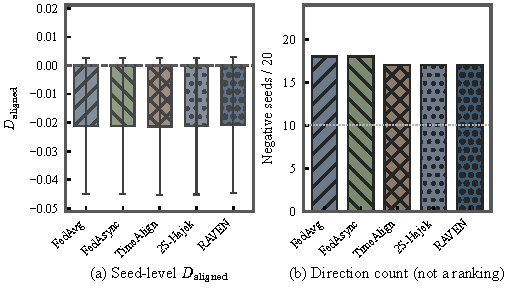
\includegraphics[width=\columnwidth]{fig2_e2_risk_noninterchangeability.pdf}
\caption{RQ1 on complete-aligned NSW-Traffic.  (a)~Seed-level
$D_{\mathrm{aligned}}=\Delta\mathrm{RMSE}_{\mu}-\Delta\mathrm{RMSE}_{\rho}$
over 20 paired seeds.  (b)~Count of negative seeds (not a method ranking).
A negative value means that the arrival-weighted risk changes more than the
deployment-target risk under the same selection shift.  Local-H\'ajek is omitted
here because E2 reports the five methods used in the risk-semantic test.}
\label{fig:risk_noninterchangeability}
\end{figure}

\noindent\textbf{Answer to RQ1.}
Yes.  The E2 result is empirical evidence for the risk-semantic distinction
formalized by Proposition~1: under structured two-stage non-random selection,
the arrival law need not be an interchangeable proxy for the intended
deployment target.  This experiment validates the problem being solved.  It is
not a RAVEN-vs-baseline superiority test.

The same four-block mismatch appears under real taxi opportunity.
Fig.~\ref{fig:g3_tdrive} compares the public H1--H4 masses with the
mass induced by processed T-Drive trajectories.  Real $R$ is
intermittent (mean client active fraction $0.425$, burstiness
$+0.38$, cell coverage $0.547$), whereas protocol Complete-aligned
$R$ on SensorScope and U-Air is always-on.  The four-block total
variation $\mathrm{TV}(\pi^{\mathrm{opp}},\boldsymbol\mu)$ is $0.142$
on T-Drive, $0.192$ on protocol SensorScope, and $0.278$ on protocol
U-Air, all above the pre-registered $0.05$ threshold.  Observation and
usable-update layers on T-Drive remain Complete-aligned controls;
this is a real-mobility opportunity replay (evidence level~A), not an
end-to-end MCS system and not a T-Drive RMSE ranking.

\begin{figure}[t]
\raggedright
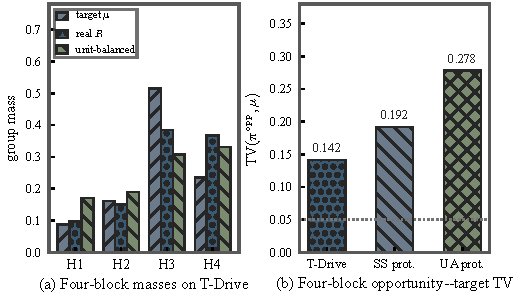
\includegraphics[width=\columnwidth]{fig_g3_tdrive_h_mass.pdf}
\caption{T-Drive real-mobility opportunity replay.  (a)~Four UTC
deployment-group masses: public target $\boldsymbol\mu$, real taxi
opportunity, and a unit-balanced reference.  Real $R$ under-serves the
afternoon block H3 and over-serves H4.  (b)~Four-block
$\mathrm{TV}(\pi^{\mathrm{opp}},\boldsymbol\mu)$ under real T-Drive
opportunity and under protocol-generated SensorScope / U-Air
opportunity.  Protocol $R$ is always-on; taxi $R$ is intermittent.
No method is ranked on T-Drive.}
\label{fig:g3_tdrive}
\end{figure}

\subsection{RQ2: Structural Alignment, Target RMSE, and Worst-Group Risk}
\label{subsec:eval_rq2}

Table~\ref{tab:main_effectiveness} reports support-conditional Design.
On SensorScope that assignment is full RAVEN (Design on).  It reduces
$\Delta_{\mathrm{group}}$/$\Delta_{c\text{-}s}$ from FedAvg's
$1.0558/1.2903$ to $1.0139/1.2644$ ($3.96\%/2.01\%$).  Four-block
worst-group RMSE is interchangeable with adapted FedAU and ObsUse
(TEST mean relative change $-0.01\%$ and $+0.05\%$).

On U-Air the assignment drops Design.  Support-conditional RAVEN obtains
$\Delta_{\mathrm{group}}=1.0165$ and $\mathrm{RMSE}_{\mu}=1.1131$,
versus $1.0924$ and $1.1911$ for full Design.  Fig.~\ref{fig:w1_design_gate}
shows why: estimated Design and oracle Design both worsen the
primaries by about $7\%$ relative to No-Design, so the reversal is
support-incompatible $\pi^{\mathrm{tar}}$, not plug-in failure.
Full Design still improves $\Delta_{c\text{-}s}$ ($1.2334$ versus
support-conditional $1.2949$) and is retained as a labeled diagnostic row.  On the
four-block worst-group endpoint, support-conditional RAVEN is non-inferior to
adapted FedAU and ObsUse (TEST $+0.48\%$ and $+0.44\%$, both inside
the $+0.5\%$ rule; Holm tests against those two are not significant).
It improves on TwoStage-H\'ajek and FedAvg (TEST $-9.11\%$ and
$-6.17\%$).  Full Design does not: its worst-group RMSE is
$1.2630$ versus FedAvg $1.2596$.  We do not claim a best
worst-group method.

The sealed same-backbone family, including FedAsync, TimeAlign,
Inst-Cal, and Debt-Cal, is in the supplemental material.  On U-Air
those RAVEN bars are full Design, not the support-conditional rows of
Table~\ref{tab:main_effectiveness}.  Local-H\'ajek coincides with
FedAvg because the realized within-client H\'ajek weights are uniform
(supplemental material).

\begin{table}[!htbp]
\centering
\caption{E3 main effectiveness (mean $\pm$ std over 20 seeds).  Lower is
better.  RAVEN-MCS (SCD) is support-conditional Design: on for
SensorScope, off for U-Air.  U-Air full Design is a diagnostic.
$\mathrm{WorstGroupRMSE}$ is the maximum error over the four UTC
deployment groups, not a finer internal grouping.  FedAU-Window and
ObsUse-Window are windowed adaptations, not official reproductions.
Support-conditional RAVEN is non-inferior to those two on worst-group RMSE
($+0.5\%$ rule); we do not claim a Holm-significant win over FedAU.
Local-H\'ajek coincides with FedAvg and is omitted.}
\label{tab:main_effectiveness}
\scriptsize
\setlength{\tabcolsep}{1pt}
\begin{tabular}{llcccc}
\toprule
Dataset & Method & $\mathrm{RMSE}_{\mu}$ & WorstGroupRMSE &
$\Delta_{\mathrm{group}}$ & $\Delta_{c\text{-}s}$\\
\midrule
\multirow{5}{*}{SensorScope}
& FedAvg-Window     & \shortstack{$7.9389$\\ $\pm0.0459$} & \shortstack{$8.6716$\\ $\pm0.0471$} & \shortstack{$1.0558$\\ $\pm0.0288$} & \shortstack{$1.2903$\\ $\pm0.0306$}\\
& TwoStage-Hajek    & \shortstack{$7.9309$\\ $\pm0.0543$} & \shortstack{$8.6633$\\ $\pm0.0556$} & \shortstack{$1.0353$\\ $\pm0.0347$} & \shortstack{$1.2910$\\ $\pm0.0324$}\\
& FedAU-Window      & \shortstack{$7.9364$\\ $\pm0.0507$} & \shortstack{$8.6691$\\ $\pm0.0522$} & \shortstack{$1.0719$\\ $\pm0.0263$} & \shortstack{$1.3057$\\ $\pm0.0313$}\\
& ObsUse-Window     & \shortstack{$7.9293$\\ $\pm0.0513$} & \shortstack{$8.6618$\\ $\pm0.0528$} & \shortstack{$1.0650$\\ $\pm0.0272$} & \shortstack{$1.3062$\\ $\pm0.0311$}\\
& RAVEN-MCS (SCD) & \shortstack{$7.9380$\\ $\pm0.0473$} & \shortstack{$8.6707$\\ $\pm0.0486$} & \shortstack{$\mathbf{1.0139}$\\ $\pm0.0305$} & \shortstack{$\mathbf{1.2644}$\\ $\pm0.0312$}\\
\midrule
\multirow{6}{*}{U-Air}
& FedAvg-Window     & \shortstack{$1.1882$\\ $\pm0.0649$} & \shortstack{$1.2596$\\ $\pm0.0709$} & \shortstack{$1.1218$\\ $\pm0.0417$} & \shortstack{$1.2621$\\ $\pm0.0309$}\\
& TwoStage-Hajek    & \shortstack{$1.2160$\\ $\pm0.0716$} & \shortstack{$1.2907$\\ $\pm0.0753$} & \shortstack{$1.1196$\\ $\pm0.0445$} & \shortstack{$1.2406$\\ $\pm0.0297$}\\
& FedAU-Window      & \shortstack{$1.1128$\\ $\pm0.0600$} & \shortstack{$1.1701$\\ $\pm0.0689$} & \shortstack{$1.0557$\\ $\pm0.0370$} & \shortstack{$1.3291$\\ $\pm0.0360$}\\
& ObsUse-Window     & \shortstack{$1.1120$\\ $\pm0.0600$} & \shortstack{$1.1692$\\ $\pm0.0689$} & \shortstack{$1.0413$\\ $\pm0.0374$} & \shortstack{$1.3235$\\ $\pm0.0349$}\\
& RAVEN (full Design) & \shortstack{$1.1911$\\ $\pm0.0659$} & \shortstack{$1.2630$\\ $\pm0.0716$} & \shortstack{$1.0924$\\ $\pm0.0479$} & \shortstack{$\mathbf{1.2334}$\\ $\pm0.0320$}\\
& RAVEN-MCS (SCD) & \shortstack{$1.1131$\\ $\pm0.0638$} & \shortstack{$1.1703$\\ $\pm0.0734$} & \shortstack{$\mathbf{1.0165}$\\ $\pm0.0458$} & \shortstack{$1.2949$\\ $\pm0.0293$}\\
\bottomrule
\end{tabular}
\end{table}

\begin{figure}[t]
\raggedright
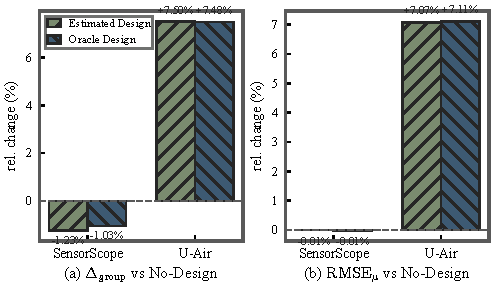
\includegraphics[width=\columnwidth]{fig_w1_design_gate.pdf}
\caption{Design versus No-Design, estimated and oracle propensities
(20 seeds; positive $=$ Design worse).  On SensorScope, Design slightly
reduces $\Delta_{\mathrm{group}}$ ($-1.23\%$ estimated, $-1.03\%$
oracle) with a flat RMSE.  On U-Air, estimated and oracle Design both
worsen $\Delta_{\mathrm{group}}$ by about $7.5\%$ and RMSE by about
$7.1\%$.  E3 therefore applies Design on SensorScope and withholds it
on U-Air.  Full Design's U-Air $\Delta_{c\text{-}s}$ gain remains in
Table~\ref{tab:e4_ablation}.}
\label{fig:w1_design_gate}
\end{figure}



These findings agree with the scope of the theory.  Proposition~2 gives
a target-law interpretation to the \emph{ideal pooled} sequential correction,
but explicitly does not claim that every finite-window reference vector exactly
equals $\boldsymbol{\mu}$.  Proposition~\ref{prop:practical_plugin}
applies only when A5 holds and $\mathcal{A}_r$ is fixed; that is the
SensorScope Design regime, not U-Air full Design.  E3 evaluates the
finite-window system after the feasibility-aware calibration in (P2).

\noindent\textbf{Answer to RQ2.}
On SensorScope, support-conditional RAVEN (Design on) consistently reduces structural
mismatch relative to FedAvg while remaining competitive on RMSE and
non-inferior on four-block worst-group RMSE.  On U-Air, the same assignment
(Design off) improves the primary endpoints and worst-group
RMSE relative to full Design and to FedAvg/TwoStage-H\'ajek, and is
non-inferior to adapted FedAU and ObsUse.  Full Design's U-Air
$\Delta_{c\text{-}s}$ gain is retained as a trade-off, not hidden.
A pre-registered under-served-block check on validation did not produce
a second external win (Section~\ref{subsec:eval_underserved}).
Traffic is excluded from this inferential conclusion.

\subsection{A Pre-Registered Under-Served-Block Check}
\label{subsec:eval_underserved}

Four-block $\mathrm{WorstGroupRMSE}$ is the maximum error over the UTC
groups that define $\boldsymbol\mu$.  That maximum can coincide with the
intrinsically hardest block rather than with the block whose public
target mass most exceeds opportunity mass.  After freezing the
support-conditional Design assignment and the worst-group look, we therefore scored a second
prediction endpoint on validation only.  The under-served block is
$g^{\star}=\arg\max_{g\in\{0,1,2,3\}}
(\mu_g-\pi^{\mathrm{opp},4}_g)$,
using the frozen public four-block target $\boldsymbol\mu$ and the
training-split opportunity law marginalized onto the same groups,
$\pi^{\mathrm{opp},4}$.  Ties take the lowest index.  The pair
$(\boldsymbol\mu,\pi^{\mathrm{opp},4},g^{\star})$ was frozen before any
method scoring; $g^{\star}$ was not chosen by inspecting per-block RMSE.
SensorScope yields $g^{\star}=2$ (12:00--18:00~UTC; gap $+0.114$);
U-Air yields $g^{\star}=3$ (18:00--24:00~UTC; gap $+0.172$).  The score
is the $\mu$-weighted RMSE on that block, already stored from the same
traces as Table~\ref{tab:main_effectiveness}.  A win requires the mean
paired relative change versus adapted FedAU \emph{and} versus ObsUse to
be at most $-0.5\%$; no-harm is at most $+0.5\%$.  Validation uses ten
paired seeds; Table~\ref{tab:underserved_block} reports the resulting
relative RMSEs.  The corresponding test seeds were not opened.

\begin{table}[t]
\centering
\caption{Validation-only under-served-block RMSE of support-conditional RAVEN relative
to adapted FedAU and ObsUse (ten paired seeds; negative means
support-conditional RAVEN is better).  A win requires both columns $\le-0.5\%$.  Neither
dataset meets that rule; both satisfy no-harm ($\le+0.5\%$).  The test
look was not opened.}
\label{tab:underserved_block}
\setlength{\tabcolsep}{3.5pt}
\begin{tabular}{lcccc}
\toprule
Dataset & $g^{\star}$ (UTC) & vs FedAU & vs ObsUse & Win / no-harm\\
\midrule
SensorScope & 2 (12--18) & $+0.05\%$ & $+0.15\%$ & No / Yes\\
U-Air & 3 (18--24) & $-0.44\%$ & $-0.27\%$ & No / Yes\\
\bottomrule
\end{tabular}
\end{table}

Neither dataset meets the win rule; both satisfy no-harm.
On SensorScope, $g^{\star}$ is the worst group.  On U-Air it is not, and
the support-conditional assignment still misses $-0.5\%$.  Informed $\mu$-weighted copies
were not trained.  Worst-group non-inferiority remains the only external
endpoint statement.

\subsection{RQ3: What Do the Correction and Calibration Components Do?}
\label{subsec:eval_rq3}

E4 removes Design, Obs, Use, Inst, or Debt one at a time under the same
Complete-aligned selection trace and paired seeds.  Fig.~\ref{fig:e4_ablation}
visualizes the one-factor removals, and Table~\ref{tab:e4_ablation}
reports the relative change
$\delta_{\mathrm{remove}}(M)
=(M_{\mathrm{ablated}}-M_{\mathrm{full}})/M_{\mathrm{full}}\times100\%$,
so a positive number means that removing the component worsens the metric.
The Inst ablation uses the one-factor removal under the same paired seeds, and
all significance statements below use the pre-specified Holm families.

\begin{table}[!htbp]
\centering
\caption{E4 relative change (\%) after removing one RAVEN component.
Positive means the ablation worsens the metric; negative means it improves the
metric.  $^\ast$ denotes Holm-adjusted $p<0.05$.}
\label{tab:e4_ablation}
\setlength{\tabcolsep}{3.5pt}
\begin{tabular}{llrrrr}
\toprule
Dataset & Removed & $\Delta_{\mathrm{group}}$ &
$\Delta_{c\text{-}s}$ & $\mathrm{RMSE}_{\mu}$ & Tail RMSE\\
\midrule
\multirow{5}{*}{SensorScope}
& Design & $+1.237^\ast$ & $+0.597^\ast$ & $+0.005$ & $+0.005$\\
& Obs    & $+0.096$       & $-0.070^\ast$ & $+0.012$ & $+0.011$\\
& Use    & $+0.026$       & $+0.026$       & $+0.012$ & $+0.012$\\
& Inst   & $-0.260$       & $+0.310^\ast$ & $-0.002$ & $-0.002$\\
& Debt   & $+0.014^\ast$ & $+0.004^\ast$ & $<0.001$ & $<0.001$\\
\midrule
\multirow{5}{*}{U-Air}
& Design & $-6.943^\ast$ & $+4.990^\ast$ & $-6.553^\ast$ & $-6.875^\ast$\\
& Obs    & $+0.123^\ast$ & $+0.022$       & $-0.010$       & $-0.010$\\
& Use    & $+0.014$       & $-0.014$       & $+0.024$       & $+0.025$\\
& Inst   & $-0.089$       & $-0.143$       & $+0.131^\ast$ & $+0.136^\ast$\\
& Debt   & $+0.004^\ast$ & $+0.002^\ast$ & $<0.001$ & $<0.001$\\
\bottomrule
\end{tabular}
\end{table}

\begin{figure}[t]
\centering
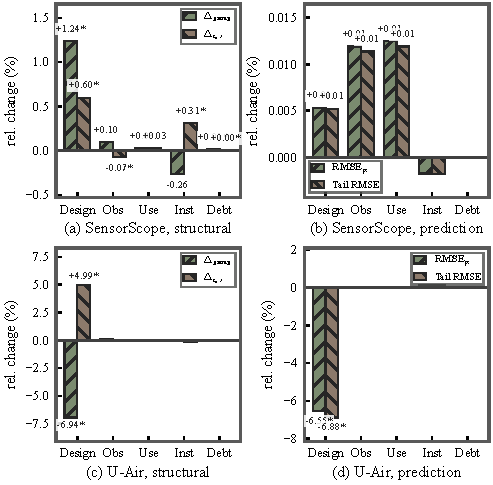
\includegraphics[width=\columnwidth]{fig5_e4_component_ablation.pdf}
\caption{RQ3 one-factor component removal.  Positive bars mean that removing the
component worsens the metric; $^\ast$ marks Holm-adjusted $p<0.05$.
(a)(b)~SensorScope structural and prediction endpoints;
(c)(d)~U-Air structural and prediction endpoints.
Values with $|\delta|<0.05\%$ and no significance mark are left unlabeled.
Sign reversals show endpoint- and dataset-dependent roles rather than
uniformly additive benefits.  A magnified U-Air non-Design view is in the supplemental material.}
\label{fig:e4_ablation}
\end{figure}

\paragraph{Design correction.}
Removing Design worsens $\Delta_{c\text{-}s}$ by $0.597\%$ on SensorScope and
$4.990\%$ on U-Air, both Holm-significant.  On U-Air the same ablation
improves $\Delta_{\mathrm{group}}$ by $6.943\%$ and
$\mathrm{RMSE}_{\mu}$ by $6.553\%$.  That reversal is why E3 withholds
Design on U-Air: Design is support-incompatible there
($25.5\%$ zero-target units; $\mathcal{A}_r$ overlap $51.6\%$), not
because estimated propensities fail
(Fig.~\ref{fig:w1_design_gate}).  Oracle Design tracks estimated
Design.  SensorScope keeps Design.  A 774-window check found identical
R/O/U and registration events, with differences beginning only at the
positive-weight/P2-support layer
(supplemental material).
The non-Design components are magnified in the supplemental material.

\paragraph{Observation and usable-update correction.}
Observation correction has a smaller, endpoint-specific effect.  On U-Air,
removing Obs worsens $\Delta_{\mathrm{group}}$ by $0.123\%$
(Holm-significant), while its $\Delta_{c\text{-}s}$ and prediction effects are
not significant.  On SensorScope, the $+0.096\%$ group change is not
significant after Holm correction, whereas
$\Delta_{c\text{-}s}$ slightly improves by $0.070\%$ when Obs is removed.
Thus Obs is best characterized as another endpoint trade-off.  In contrast,
removing Use produces no significant change in any of the four core endpoints
on either dataset.  E4 therefore does not establish the marginal
indispensability of usable-update correction in this Complete-aligned family;
the theoretical selection layer remains distinct, but its isolated empirical
effect is not clearly established here.

\paragraph{Instantaneous calibration and debt.}
Inst also exhibits a trade-off.  On SensorScope, removing it worsens
$\Delta_{c\text{-}s}$ by $0.310\%$ (significant), while the
$-0.260\%$ change in $\Delta_{\mathrm{group}}$ is not significant after Holm
correction.  On U-Air, the small structural
changes are not significant, but removing Inst worsens
$\mathrm{RMSE}_{\mu}$ and tail RMSE by $0.131\%$ and $0.136\%$,
respectively (both $p_{\mathrm{Holm}}=0.0194$).  Hence Inst exhibits an
endpoint trade-off, rather than a purely structural role.

Debt has the narrowest but most consistent role.  Removing it significantly
increases both structural mismatches on both datasets, but only by
$0.0141\%/0.0040\%$ on SensorScope and
$0.0043\%/0.0024\%$ on U-Air, well below the $0.5\%$ paired-relative
minimum practical effect used elsewhere; prediction changes are negligible.
This matches long-term accounting in \eqref{eq:debt_bound}, not a
standalone performance driver, and does not establish
$\|\mathbf Q_R\|_1=o(S_R)$.

\noindent\textbf{Answer to RQ3.}
RAVEN is a coupled correction-and-calibration system, not five monotone
boosters.  As a reconstruction factor, Design helps SensorScope and
reverses U-Air primaries while still buying $\Delta_{c\text{-}s}$.
Obs has weaker endpoint-specific effects.  Usable-update correction is
kept as a sequential selection layer; E4 does not show an isolated
effect.  Inst trades finite-window structure against prediction.
Target debt is a consistent accounting term whose isolated changes stay
well below the $0.5\%$ practical threshold.

\subsection{Finite-Sample Audit of the Aggregate Coverage Certificate}
\label{subsec:eval_certificate}

RAVEN-MCS switches Design by target-support compatibility
(Algorithm~\ref{alg:window_close}).  This subsection audits a candidate
per-window coverage Gate (Algorithm~\ref{alg:agg_certificate}) on a frozen
coverage-stress oracle that supplies realized aggregate coverage $C_t$
only after each window closes.  The Gate uses only legal pre-window
features $F_{t-}$.

Availability levels are $a\in\{1.00,0.80,0.60,0.40,0.20\}$ on the
SensorScope and U-Air test tracks (62 and 53 windows).  A ridge predictor
with unpenalized intercept, penalty $1.0$, public $a_t$, two lags of $C$,
an $L=8$ rolling mean and linear trend, and hour/weekend encodings is
fit once on the corresponding training-split pretest windows (187 on
SensorScope, 158 on U-Air) and then frozen.  Calibration buffers start
empty.  After a completed CERTIFIED window, RESET occurs if
$C^{\mathrm{LCB}}>C$; that window is retained, and the next window is
RESET then a new-block WARMUP.  The constants remain $n_{\min}=19$,
$\alpha=0.05$, and $\tau_{\mathrm{cov}}=0.05$.

Table~\ref{tab:certificate_stress} reports the ten tracks.
Across $575$ scored windows, $243$ are CERTIFIED.  Pooled empirical
validity is $0.959$ ($10$ miscoverages) with zero false-safe Gate
openings.  The Clopper--Pearson one-sided $95\%$ upper bound on pooled
miscoverage is $0.069$; these intervals are reporting quantities and do
not prove Assumption~\ref{ass:score-exchangeability}.
Theorem~\ref{thm:agg-lcb} remains conditional on that assumption.

On SensorScope with $a=0.40$, the median LCB is $0.041$, below
$\tau_{\mathrm{cov}}$, so Gate stays off on every window even though
$24$ windows are CERTIFIED and empirical validity is $0.958$
(Fig.~\ref{fig:certificate_audit}b).  On U-Air with $a=0.20$ the median
LCB is $0.013$ and validity is $1.000$; Gate is likewise never on.
On U-Air with $a=1.00$ the eight CERTIFIED windows have empirical
validity $0.750$, so that track does not establish the nominal $95\%$
certificate.  Those miscoverages need not be false-safe openings.
$C$ can remain at least $\tau_{\mathrm{cov}}$ while
$C^{\mathrm{LCB}}$ still exceeds $C$.  Fig.~\ref{fig:certificate_audit}a shows the CERTIFIED
$(C_t,C^{\mathrm{LCB}}_t)$ pairs.  Points above the diagonal are
miscoverages; points below the horizontal line at $0.05$ keep Gate off.

The audit therefore characterizes a conservative candidate Gate at
$\tau_{\mathrm{cov}}$, including a U-Air natural-availability validity
failure.  Tables~\ref{tab:main_effectiveness}--\ref{tab:e4_ablation}
continue to report support-conditional Design.

\begin{table*}[t]
\centering
\caption{Coverage-stress audit of a candidate aggregate coverage Gate.
Validity is the fraction of CERTIFIED windows with
$C^{\mathrm{LCB}}\le C$.  FSR is the false-safe rate among CERTIFIED
windows with $C<\tau_{\mathrm{cov}}$.  Gate ON is the fraction of all
windows with $\mathrm{Gate}_t=1$.  SensorScope $a=0.40$ and U-Air
$a=0.20$ keep Gate off because the LCB stays below $\tau_{\mathrm{cov}}$.
U-Air $a=1.00$ misses the nominal $95\%$ empirical validity.}
\label{tab:certificate_stress}
\scriptsize
\setlength{\tabcolsep}{3.2pt}
\begin{tabular}{lcccccccc}
\toprule
Dataset & $a$ & $n$ & $n_{\mathrm{cert}}$ & Duty & Validity & FSR & Gate ON & Median $C^{\mathrm{LCB}}$\\
\midrule
\multirow{5}{*}{SensorScope}
& $1.00$ & $62$ & $43$ & $0.694$ & $1.000$ & $0.000$ & $0.694$ & $0.124$\\
& $0.80$ & $62$ & $29$ & $0.468$ & $0.966$ & $0.000$ & $0.452$ & $0.093$\\
& $0.60$ & $62$ & $24$ & $0.387$ & $0.958$ & $0.000$ & $0.306$ & $0.065$\\
& $0.40$ & $62$ & $24$ & $0.387$ & $0.958$ & $0.000$ & $0.000$ & $0.041$\\
& $0.20$ & $62$ & $24$ & $0.387$ & $0.958$ & $0.000$ & $0.000$ & $0.017$\\
\midrule
\multirow{5}{*}{U-Air}
& $1.00$ & $53$ & $8$ & $0.151$ & $0.750$ & $0.000$ & $0.151$ & $0.182$\\
& $0.80$ & $53$ & $11$ & $0.208$ & $0.818$ & $0.000$ & $0.208$ & $0.129$\\
& $0.60$ & $53$ & $15$ & $0.283$ & $0.933$ & $0.000$ & $0.245$ & $0.093$\\
& $0.40$ & $53$ & $31$ & $0.585$ & $0.968$ & $0.000$ & $0.340$ & $0.051$\\
& $0.20$ & $53$ & $34$ & $0.642$ & $1.000$ & $0.000$ & $0.000$ & $0.013$\\
\bottomrule
\end{tabular}
\end{table*}

\begin{figure}[t]
\raggedright
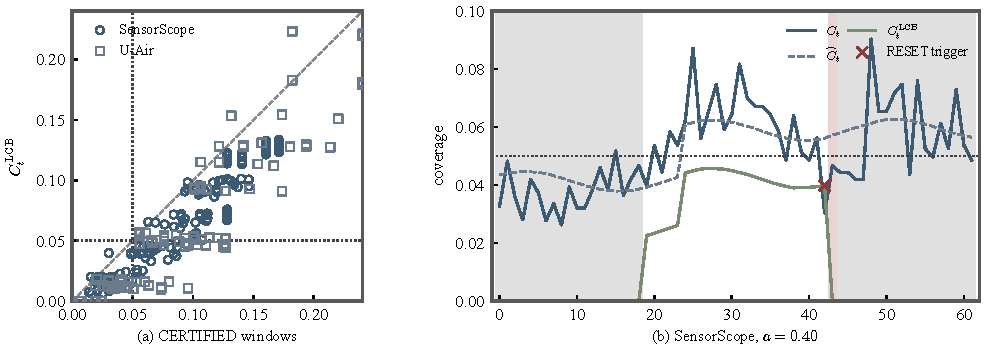
\includegraphics[width=\columnwidth]{fig_certificate_audit.pdf}
\caption{Finite-sample audit of the aggregate coverage certificate.
(a)~CERTIFIED windows: realized coverage $C_t$ versus
$C^{\mathrm{LCB}}_t$.  The dashed line is $y=x$; dotted lines mark
$\tau_{\mathrm{cov}}=0.05$.
(b)~SensorScope $a=0.40$ timeline.  Gray bands are WARMUP; the red mark
is a retained CERTIFIED miscoverage that triggers RESET on the next
window.  The LCB stays below $0.05$, so Gate remains off.}
\label{fig:certificate_audit}
\end{figure}

\section{Discussion and Limitations}
\label{sec:discussion}

RAVEN-MCS aligns windowed-asynchronous federated completion with a public
deployment target.  The claim is not universal RMSE dominance.
Design is applied when target support is compatible and withheld when it
is not.  Structural metrics measure target alignment directly; prediction
risk must remain competitive.

\subsection{Support-Conditional Design and the U-Air Reversal}
\label{subsec:discussion_gate}

On SensorScope, Design slightly improves both structural endpoints
without an RMSE cost.  On U-Air, full Design improves
$\Delta_{c\text{-}s}$ while worsening $\Delta_{\mathrm{group}}$,
RMSE, tail RMSE, and four-block worst-group RMSE by about $7\%$.
Oracle Design tracks estimated Design, so the reversal is
support-incompatible $\pi^{\mathrm{tar}}$: $25.5\%$ of risk units
have zero target mass, and $\mathcal{A}_r$ changes.  It is not a failure of
plug-in propensities.  Proposition~\ref{prop:practical_plugin} does
not apply in that regime: A5 requires positivity on target support and
a common active set.  A support-compatible mixture target was tested as
a universal repair and failed the SensorScope do-not-break rule; it is
not a hidden method.  Withholding Design on U-Air is the RAVEN-MCS
assignment.  Section~\ref{subsec:eval_certificate} audits a candidate
coverage Gate that is not used in E3: at SensorScope $a=0.40$ and
U-Air $a=0.20$ that Gate stays off, and U-Air $a=1.00$ does not
establish the nominal $95\%$ empirical validity.

The same trade-off explains why structural alignment need not move RMSE
one-for-one.  Proposition~1 distinguishes the two risk functionals;
Proposition~2 identifies the ideal pooled correction, not every
finite-window $\boldsymbol\beta_r$.  On U-Air, withholding Design also
improves RMSE; on SensorScope the RMSE change is negligible.  Adapted
FedAU and ObsUse remain the strong participation comparators on
four-block worst-group RMSE.  Support-conditional RAVEN is non-inferior to both under
the pre-registered $+0.5\%$ rule.  We do not claim a best worst-group
method, and FedCure was not run.  The under-served-block check remains a
recorded negative; it did not reopen Design on U-Air.

\subsection{Mobility, Identification, and Privacy}
\label{subsec:discussion_boundaries}

T-Drive supplies a real-mobility opportunity process (evidence
level~A): $R$ is trajectory-derived, while $O$ and $U$ stay
Complete-aligned controls.  Real taxi $R$ is intermittent; protocol
$R$ on SensorScope and U-Air is always-on.  The four-block
target--opportunity mismatch has the same sign in all three traces.
This is not an end-to-end system, not real federated updates, and not a
T-Drive ranking.  Original SensorScope and U-Air traces are not claimed
to contain mobile clients.

A1--A2 remain modeling boundaries: RAVEN does not recover mass outside
opportunity support and does not correct arbitrary hidden confounding.
If $h(i)$ or $s(i)$ is misspecified, calibration tracks the wrong
target.  Proposition~\ref{prop:practical_plugin} is a stability
statement for the clipped plug-in when A5 holds; it is not
unbiasedness, and $C_1$ is not a tight RMSE certificate.

Propensity covariates can include location, network state, and device
availability.  RAVEN uses only lagged pre-outcome histories, does not
centralize raw records, and needs only aggregated selection statistics
at the server.  Collecting those metadata still has a privacy cost;
deployments should minimize the covariate set and retain aggregated
rather than per-event features where possible.

\subsection{Evidence Scope}
\label{subsec:discussion_evidence_limits}

NSW-Traffic is RQ1 evidence only; it is not used to rank methods.
Local-H\'ajek equals FedAvg on these blocks because within-client
weights are uniform (supplemental material), a
protocol-specific degeneracy rather than a general equivalence.
P2 outputs are feasibility-certified
(supplemental material); exact post-hoc optimality of every
solve is not claimed.  On later reconstructable logs, CLARABEL and SCS
typically match to $10^{-8}$ in $\ell_1$, with a worst-window
allocation gap of $0.0056$ that does not move the E3 headlines.  A window-level $10^{-4}/10^{-3}$ divergence rule is
recorded; the stored P2 outputs were not re-solved under a different solver.

The $20$ seeds are algorithmic and EventTrace randomness, not
independent cities.  Debt effects of $0.002\%$--$0.014\%$ are
quantitatively small relative to the $0.5\%$ practical threshold even
where $p<0.05$.  U-Air Design-off remains a practically meaningful
effect under that same threshold.  The under-served-block percentages
are validation-only; they are not a test ranking and do not reopen
Design on U-Air.


\section{Conclusion}
\label{sec:conclusion}

Windowed-asynchronous federated MCS completion should align selected
mass with the public deployment target, not with the arrival law of
usable updates.  RAVEN-MCS separates that target from the R/O/U
selection process, reconstructs target-relevant mass from legal
pre-outcome histories, and calibrates the reference inside the current
feasible window, carrying residual group under-service as target debt.
When the deployment and arrival laws differ, their risks are not
interchangeable.  The ideal sequential correction recovers the
compatible target under support and identification conditions; the
calibration program is uniquely solvable; and the clipped plug-in is a
stable perturbation of the same-window ideal reference when target
support is compatible.

RAVEN-MCS applies Design when the public target has compatible support
and withholds it when that support fails, as on U-Air.  A finite-sample
aggregate coverage bound is stated in Theorem~\ref{thm:agg-lcb}.  On a
coverage-stress oracle the associated Gate has pooled empirical validity
$0.959$ and zero false-safe openings, but it is conservative at
$\tau_{\mathrm{cov}}$ and does not establish $95\%$ validity on U-Air
natural availability.  E3 therefore keeps support-conditional Design.
The under-served-block check on validation did not beat adapted FedAU and
ObsUse by $0.5\%$, so the test look was not opened.  Real T-Drive taxi
opportunity reproduces the four-block
mismatch without supplying a method ranking.  Usable-update correction has no clear isolated effect in the tested
family.  Target debt remains internal accounting; its isolated changes
are quantitatively small.

These guarantees hold under explicit support and sequential
identification.  They do not cover arbitrary hidden confounding,
misspecified targets, or end-to-end mobile systems.  SensorScope and U-Air
ranking results use protocol opportunity.  Extending the T-Drive replay to
jointly measured observation and network processes remains future work.

Proofs, additional tables, runtime measurements, and the sealed
same-backbone E3 plots are submitted as a separate supplemental PDF
and are not part of this file.

\section*{Data and Code Availability}
The SensorScope, U-Air, NSW-Traffic, and T-Drive sources are public
and cited in Section~\ref{subsec:eval_setup}.  A frozen public
reproducibility bundle is released with this paper as
\texttt{RAVEN\_MCS\_PUBLIC\_REPRO\_R1}.  It contains the paired seeds,
frozen target maps, selection-protocol configs, EventTrace files and
indexes, tabulated results used by the figures and tables, and the
coverage-audit window records.  A verifier in that directory checks
file hashes against the included manifest.  FedAU-Window and
ObsUse-Window are windowed adaptations, not official reproductions of
those systems.  GPU-scale 20-seed retraining is not required to verify
the tabulated numbers.

\bibliographystyle{IEEEtran}
\bibliography{reference}

\end{document}
